\documentclass[a4paper,oneside,11pt]{report}

%------------ package pour langue fr ------
\usepackage[utf8]{inputenc}
\usepackage[french]{babel}
\usepackage[T1]{fontenc}
\usepackage{multicol}
\usepackage{enumitem}
\usepackage{multirow}
%------------- for embedding images----------
\usepackage{graphicx} 
\usepackage{float}
\usepackage[export]{adjustbox}
\usepackage{amsfonts,epsfig,epstopdf,titling,url,array}
\usepackage{lscape}

\usepackage{amsmath}
\usepackage{amssymb}
\usepackage{amsthm}
%--------- pour le style de la page ----------
\usepackage[top=3cm, bottom=3cm, left=2.5cm, right=2cm]{geometry}

\usepackage[]{geometry}

\usepackage{algorithm}
\usepackage{algorithmic}


\usepackage{setspace}
\setstretch{1,5}
%\usepackage{txfonts} //pour utiliser times new roman dans le document
\usepackage{fancyhdr}
\pagestyle{fancy}
%\renewcommand\headrulewidth{1pt}
%\fancyhead[L]{Bousbiat Hafsa - Ihadadene Sana}
%\fancyhead[R]{Rapport Master}
%--------------------------- Sommaire ----------------------------%
\usepackage{hyperref}
\usepackage{amssymb}
\usepackage{natbib}
\theoremstyle{definition}
		\newtheorem{defn}{Definition}[section]
		\newtheorem{conj}{Conjecture}[section]
		\newtheorem{exmp}{Example}[section]
\usepackage[table,dvipsnames]{xcolor}	

\usepackage{pifont}% http://ctan.org/pkg/pifont
\newcommand{\xmark}{\color{red}\ding{55}}%
\newcommand{\cmark}{\color{PineGreen}\ding{51}}	
\usepackage[T1]{fontenc}
\newcolumntype{R}[1]{>{\raggedleft\arraybackslash }b{#1}}
\newcolumntype{L}[1]{>{\raggedright\arraybackslash }b{#1}}
\newcolumntype{C}[1]{>{\centering\arraybackslash }b{#1}}


\begin{document}

%Page de garde (page de titre)							Obligatoire

\begin{titlepage}

\newgeometry{top=0mm,right=20mm,left=20mm,bottom=0mm}



	%--------------------  Entete de l'Ecole ----------------------%

	\begin{figure}[t]
		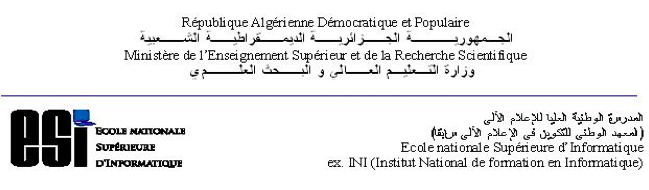
\includegraphics[scale=0.75]{./ressources/image/ESI.png}\\[0.6in]
	\end{figure}
	
	
	
	%--------------------------------------------------------------%
	\begin{center}
	
	%------------------------  Le sujet ---------------------------%
		\LARGE \textbf{ Mémoire}\\
		\Large{
			Pour Obtention du diplôme de Master En Informatique\\
			\textbf{Option : Système Informatique (SIQ)}
			%\textsc thèse D'Ingéniorat En Informatique sous le thème :
		}\\[0.2in]
		\huge {
		\rule{\linewidth}{.5pt}
			\textbf{
				Étude et classification des méthodes de compression de graphe par extraction de motifs et k2-trees
			} 
			\rule{\linewidth}{.5pt}
		}\\[0.5in]
		\Large
	%--------------------------------------------------------------%	
	
	%-------------------------  Mon nom ---------------------------%
	\textbf{Réaliser par:}\\
	\begin{multicols}{2}
			\Large 	Mlle. Hafsa Bousbiat\\
			\large eh\_bousbiat@esi.dz\\
			ESI\\
		\columnbreak
 			\Large Mlle. Sana Ihadadene\\
			\large es\_ihadadene@esi.dz\\
			ESI \\
		
	\end{multicols} 
	
	\vskip 0.1in
	%--------------------------------------------------------------%	

	%-----------------------  Encadreures -------------------------%
	 \textbf{Encadrer par:}\\
	 
	 \begin{multicols}{2}
			\Large 	Dr. Karima Amrouche\\
			\large k\_amrouche@esi.dz\\
			ESI\\
		\columnbreak
 			\Large Dr. Hamida Seba\\
			\large hamida.seba@univ-lyon1.fr\\
			Université de Lyon \\
	\end{multicols}
	
	%--------------------------------------------------------------%	
	
	\small
	\vskip 0.3in
	Octobre 2018 \\
	Année Universitaire: 2018-2019\\
	
	\end{center}		
\restoregeometry
\end{titlepage}

%Remerciements											Obligatoire
\begin{center}
	\par
	\textit{
		\vskip 1in
		\Huge 
			Remerciement \\[0.5in]
			\addcontentsline{toc}{chapter}{\numberline{}Remerciement}
	}
\end{center}
	\par
  Nous tenons d'abord à exprimer notre gratitude à l'égard de nos encadrants, Madame Seba
Hamida, Madame Amrouche Karima et Monsieur Mohammed pour leur précieuse	aide, leur judicieux conseils  et pour le temps qu'ils nous ont consacré tout au long de ce PFE.\\


Nous remercions également toute l'équipe pédagogique de l'École Nationale
Supérieure d'Informatique, et à leur tète les enseignants pour la richesse et la qualité de la formation qu'ils nous ont offert tout au long de notre cursus.\\


Nous tenons à remercier les membres du jury qui nous ont fait l’honneur d’accepter de juger
cet humble travail.\\


Enfin, nous adressons nos plus sincères remerciements à tous nos proches et amis, qui nous ont toujours encouragée au cours de la réalisation de ce mémoire.
Merci à tous et à toutes.

\newpage
 


%Résumé												Obligatoire
\begin{center}
	\par
	\textbf{
		\vskip 0.5in
		\LARGE 
			Résumé \\[0.15in]
			\addcontentsline{toc}{chapter}{\numberline{}Résumé}
	}
\end{center}
	\par
    Lorem ipsum dolor sit, amet consectetur adipisicing elit. Nostrum tempore ea fugiat numquam autem saepe quas porro vitae? Fugit commodi tempore voluptate sint fugiat, possimus optio ad! Pariatur, obcaecati quidem.
Lorem ipsum dolor, sit amet consectetur adipisicing elit. Neque excepturi ducimus accusantium eius voluptatibus, quod velit, explicabo tenetur aliquid ipsam sapiente. Quibusdam quis ullam, saepe numquam molestias nobis recusandae labore?    Lorem ipsum dolor sit, amet consectetur adipisicing elit. Nostrum tempore ea fugiat numquam autem saepe quas porro vitae? Fugit commodi tempore voluptate sint fugiat, possimus optio ad! Pariatur, obcaecati quidem.
Lorem ipsum dolor, sit amet consectetur adipisicing elit. Neque exceptu 

\begin{center}
	\par
	\textbf{
		\vskip 0.5in
		\LARGE 
			Abstract \\[0.15in]
	}
\end{center}
	\par
    Lorem ipsum dolor sit, amet consectetur adipisicing elit. Nostrum tempore ea fugiat numquam autem saepe quas porro vitae? Fugit commodi tempore voluptate sint fugiat, possimus optio ad! Pariatur, obcaecati quidem.
Lorem ipsum dolor, sit amet consectetur adipisicing elit. Neque excepturi ducimus accusantium eius voluptatibus, quod velit, explicabo tenetur aliquid ipsam sapiente. Quibusdam quis ullam, saepe numquam molestias nobis recusandae labore?    Lorem ipsum dolor sit, amet consectetur adipisicing elit. Nostrum tempore ea fugiat numquam autem saepe quas porro vitae? Fugit commodi tempore voluptate sint fugiat, possimus optio ad! Pariatur, obcaecati quidem.
Lorem ipsum dolor, sit amet consectetur adipisicing elit. Neque exceptu

\newpage

%Sommaire (Table des matières)							Obligatoire
\tableofcontents
\newpage

%Liste des figures										Selon besoin
\listoffigures
\addcontentsline{toc}{chapter}{\numberline{}Liste des figures}
\cleardoublepage

%Liste des tableaux										Selon besoin

\listoftables
\addcontentsline{toc}{chapter}{\numberline{}Liste des tableaux}
\cleardoublepage

%Introduction (début de la pagination)					bligatoire


\chapter{Introduction} 


%---->chapitre 01 :« cadrage du projet »
	\chapter{ Théorie des graphes}
	  Pour faciliter la compréhension d'un problème, nous avons tendance à  le dessiner ce qui nous amène parfois même à le résoudre. La théorie des graphes est fondée à l'origine sur ce principe. De nombreuses propriétés et méthodes ont été pensées ou trouvées à partir d'une représentation schématique pour être ensuite formalisées et prouvées.


La théorie des graphes est historiquement un domaine mathématique qui s'est développé  au sein des autres disciplines comme la chimie, la biologie, la sociologie et l'industrie. Elle constitue aujourd'hui un corpus de connaissance très important et un instrument efficace pour résoudre une multitude de problèmes.


De manière générale, le graphe sert à représenter les structures, les connexions entre différents composants, les acheminements possibles pour un ensemble complexe composé d'un grand nombre de situations en exprimant les dépendances et les relations entre ses éléments,(e.g. réseau routier ou ferroviaire, réseau de communication, diagramme d'ordonnancement, ..). 


Dans ce chapitre, nous présenterons les notions et les concepts clés relatives aux graphes qui serviront de base pour la suite de notre travaille, à savoir : la définition d'un graphe, ses types et sa représentation structurelle. Nous clôturons le chapitres avec quelques domaines d'application des graphes.

	
	\section{Graphe non orienté}
			\subsection{Définitions et généralités}
		
Un graphe non orienté G est la donnée d’un couple (V , E) où V = \{$ \textit{v}_{1} , \textit{v}_{2} ,..., \textit{v}_{n} $\} est un ensemble fini dont les éléments sont appelés sommets ou nœuds ( Vertices en anglais ) et  E=\{$\textit{e}_{1} ,  \textit{e}_{2} ,…, \textit{e}_{m} $\} est un ensemble fini d'arêtes ( Edges en anglais ). Toute arête \textit{e} de E correspond à un couple non ordonné de sommets ( $\textit{v}_{i} , \textit{v}_{j}$ ) $\in$ E $\subset$  $V \times V$ représentant ses extrémités \citep{muller} \citep{fages2014exploitation}.
\\Soient \textit{e} = ($\textit{v}_{i} , \textit{v}_{j}$) et \textit{e'}=($\textit{v}_{k} , \textit{v}_{l}$) deux arêtes de E, On dit que :
\begin{itemize}
\item $\textit{v}_{i}$ et $\textit{v}_{j}$ sont les extrémités de \textit{e} et \textit{e} est incidente à $\textit{v}_{i}$ et $\textit{v}_{j}$ \citep{hennecart2012elements}.
\item $\textit{v}_{i}$ et $\textit{v}_{j}$ sont voisins ou adjacents, s'il y a au moins une arête entre eux dans E \citep{IUTLyonInformatique}.
\item L'ensemble des sommets adjacents aux deux extrémités de \textit{e} est appelé le voisinage de \textit{e} \citep{muller}. 
\item \textit{e} et \textit{e'} sont voisins s'ils ont une extrémité commune  \citep{lopez2003cours}.
\item L'arête \textit{e} est une boucle si ses extrémités coïncident, i.e, $\textit{v}_{i}$ = $\textit{v}_{j}$ \citep{IUTLyonInformatique}. 
\item L'arête \textit{e} est multiple si elle a plus d'une seule occurrence dans l'ensemble E.
\end{itemize}	
		 
\subsection{Représentation graphique}
Un graphe non orienté G peut être représenté par un dessin sur un plan comme suit \citep{muller}:

\begin{itemize}
\item Les nœuds $\textit{v}_{i}$ $\in$ V de G sont représentés par des points distincts.
\item 	Les arêtes \textit{e} = ($\textit{v}_{i}$,$\textit{v}_{j}$) $\in$ E de G sont représentés par des lignes, pas forcement rectilignes, qui relient les extrémités de chaque arête \textit{e}.
\end{itemize}

%% L'exemple de la représentation graphique 
\textbf{Exemple :}
 Soit g=(V1 , E1) un graphe non orienté tel que : V1=\{ 1,2,3,4,5 \} et E1=\{(1,2), (1,4), (2,2), (2,3), (2,5), (3,4)\}.
La représentation graphique de g est alors donnée par le schéma de la figure \ref{graphNonOriente}.
\\
\begin{figure}[H]
\begin{center}
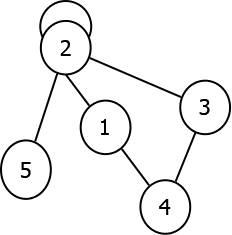
\includegraphics[height=120 pt, width=130 pt]{./ressources/image/graphNonOriente.png} 
\end{center}
\caption{Exemple de représentation graphique d'un graphe non orienté}
\label{graphNonOriente}
\end{figure}

		\subsection{Propriétés d'un graphe}
		
		\begin{itemize}[label=$\circ$]
			
			\item \textbf{Ordre d'un graphe:} On appelle ordre d’un 					graphe le nombre de ses sommets, i.e, Card(V) \citep{DUT}.
			
			\item  \textbf{Taille d'un graphe:} On appelle taille d’un 				graphe le nombre de ses arêtes, i.e, Card(E) \citep{DUT}.
			
			\item  \textbf{Degré dans un graphe:}
			
			
			\begin{itemize}[label=$\bullet$]
				\item \textbf{Degré d'un sommet : } Le degré d’un sommet noté \textit{d}($\textit{v}_{i}$) est le nombre d'arêtes incidentes à ce sommet, sachant qu’une boucle compte pour deux \citep{muller}. Dans l'exemple de la figure \ref{graphNonOriente}, le degré du sommet (1) est : \textit{d}(1)=2.
				
				\item \textbf{Degré d'un graphe : }Le degré d’un graphe est le degré maximum de ses sommets, i.e, max(\textit{d}($\textit{v}_{i}$)) \citep{muller}. Dans l’exemple de 				la figure \ref{graphNonOriente}, le degré du graphe g est \textit{d}(2)=5.
			\end{itemize}
			
			\item \textbf{Rayon et diamètre dans un graphe:}
			\begin{itemize}[label=$\bullet$]
				\item \textbf{Distance : }La distance entre deux sommets 	\textit{v} et \textit{u} est le plus petit nombre d’arêtes qu’on doit parcourir pour aller de \textit{v} à \textit{u} ou de \textit{u} à \textit{v} \citep{muller}. 
				
				\item 	\textbf{Diamètre d’un graphe :} C’est la plus grande 	distance entre deux sommets de ce graphe \citep{muller}. 
				
				\item 	\textbf{Rayon d’un graphe : }C’est la plus petite distance entre deux sommets de ce graphe \citep{parlebas1972centralite}. 
			\end{itemize}
		\end{itemize}
		
	
			
	
			
	\section{Graphe orienté}	
		
		\subsection{Définitions et généralités}
		Un graphe orienté G est la donnée d'un couple (V , E) où
		V est un ensemble fini dont les éléments sont appelés les sommets de G et 
		E  $\subset$ V x V est un ensemble de couples ordonnés de sommets dits arcs ou arêtes \citep{muller}. G est appelé dans ce cas digraphe (directed graph).\\
		 Pour tout arc e = ( $v_{i}$ , $v_{j}$) $\in$ E :
		 \begin{itemize}  
			\item $v_{i}$ est dit extrémité initiale ou origine de e et $v_{j}$ est l'extrémité finale de e \citep{muller}.
			
			\item $v_{i}$ est le prédécesseur de $v_{j}$ et $v_{j}$ est le successeur de $v_{i}$ \citep{IUTLyonInformatique}.
			
			\item les sommets $v_{i}$ , $v_{j}$ sont des sommets adjacents \citep{Pres}.
			
			\item e est dit sortant en $v_{i}$ et incident en $v_{j}$ \citep{Pres}.
			
			\item e est appelé boucle si $v_{i}$ = $v_{j}$, i.e l'extrémité initiale et finale représente le même sommet \citep{IUTLyonInformatique}.
			
		\end{itemize}
		 
		
		\subsection{Représentation graphique}
		
		
		Un graphe G = (V , E) peut être projeter sur le plan en représentant:
		\begin{itemize} 
		\item Dans un premier temps les nœuds $v_{i}$ $\in$ V par des points disjoints du plan.
		\item Et dans un second temps les arêtes e = ( $v_{i}$ , $v_{j}$) $\in$ E par des lignes orientées reliant par des flèches les deux extrémités de e. 
		\end{itemize}
		
		\textbf{Exemple:}
		
		Soit g = ($V_{1}$ , $E_{1}$) un digraphe tel que : $V_{1}$ = \{ 1,2,3,4 \} et  $E_{1}$ = \{(1,2),(1,3),(3,2),(3,4),(4,3)\}.
		
		Le représentation graphique de g est alors donné par le schéma de la figure \ref{grapheOr}.
	
		
			\begin{figure}[h]
			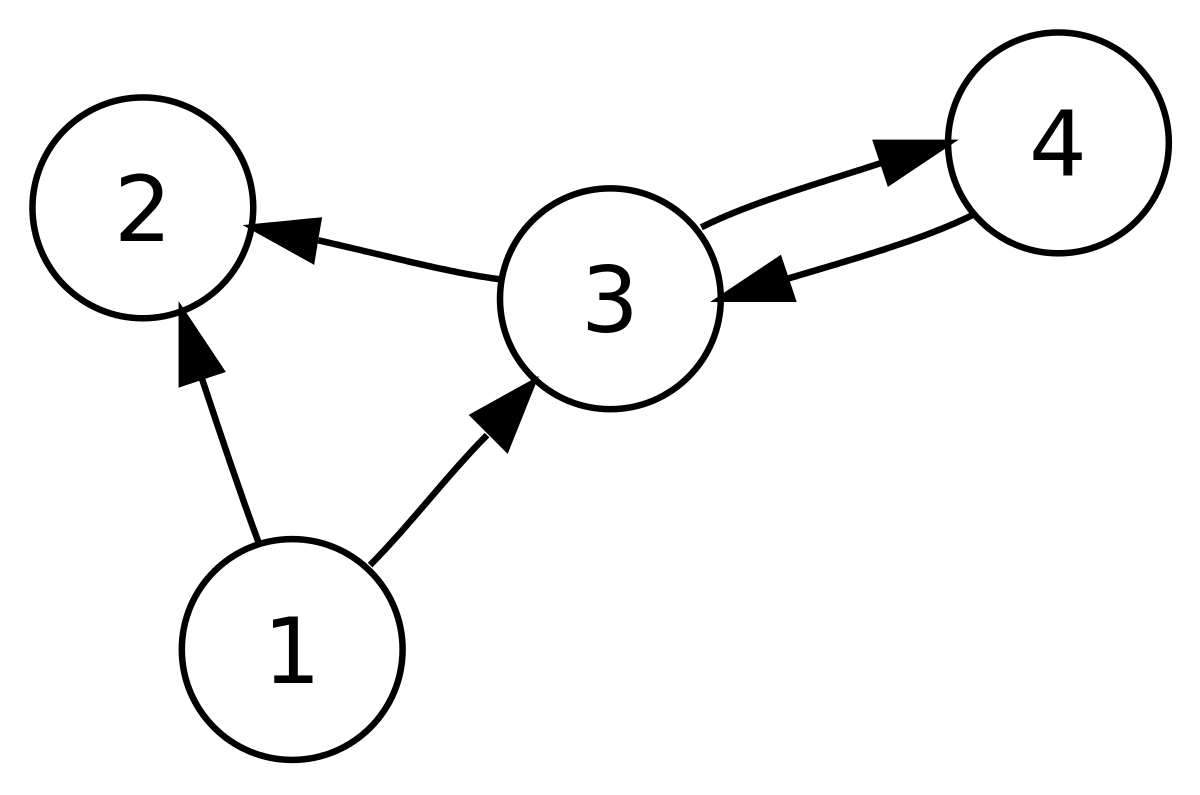
\includegraphics[scale=0.15,center]{./ressources/image/RepDiGraphe.png}
			\caption[Exemple de représentation graphique d'un digraphe.]{Exemple de représentation graphique d'un digraphe.}
			\label{grapheOr}
			\end{figure}
			
		
		\subsection{Quelques Propriétés:} %%% Arevoire 
			\begin{itemize}[label=$\circ$]
			\item\textbf{Ordre d'un digraphe:}
			est le nombre de sommets n = Card(V) \citep{DUT}.
			
			\item\textbf{taille d'un digraphe:} est le nombre d’arcs m = Card(A) \citep{DUT}.
			
			\item\textbf{Degré dans un digraphe:}
			Le degré d'un sommet $v_{i}$ $\in$ V dans un digraphe G=(V , E) est donnée par la formule :
			\begin{center}
				d($v_{i}$) = $d^+(v_{i}$) + $d^-(v_{i}$\\
			\end{center}			 
			 où $d^+(v_{i}$) est le nombre d'arcs sortants au sommet $v_{i}$ et est appelé degré extérieure et $d^-(v_{i}$) représente le nombre d'arcs incidents et est appelé degré intérieur \citep{muller}.
			 
			 \item\textbf{Voisinage dans un digraphe:}
			 Le voisinage d'un sommet $v_{i}$ $\in$ V, noté V($v_{i}$), dans un digraphe G = (V , E) est:
			 	\begin{center}
				V($v_{i}$) = succ($v_{i}$) $\bigcup$ pred($v_{i}$),
				\end{center}
				
				où succ($v_{i}$) est l'ensemble des successeurs de $v_{i}$ et pred($v_{i}$) est l'ensemble de ses prédécesseurs \citep{bac}, i.e le voisinage de $v_{i}$ est l'ensemble des sommets qui lui sont adjacents.
			
			\end{itemize}
			
		
	\section{Notion de Connexité}
	
	Les structures de graphes sont généralement exploitables à travers leurs interrogation qui permet de fournir des réponses aux problèmes modélisés. L'un des informations les plus importantes dans un graphe est la notion des relations (indirectes ou indirecte) entre deux nœuds ou plus formellement la connexité dans un graphe. Dans cette partie nous allons définir les concepts relatives à cette notion.
	
	\begin{itemize} [label = $\bullet$]
		
			 
			 \item \textbf{Chemin (resp. Chaine):}
			est une liste de sommets S= $(v_{0},v_{1},v_{2},...,v_{k})$ telle qu’il existe un arc (resp. une arête) entre chaque couple de sommets successifs.
			 
			 
			  \item \textbf{Cycle (resp. Circuit):} 
			 est un chemin (resp. chaine) dont le premier et le dernier sommet sont identiques \citep{DUT}.
			 
			 		\item \textbf{Graphe connexe:}
			Un graphe non orienté (resp. orienté) est dit connexe (resp. fortement connexe) si pour tout pair de sommets ($v_{i}$, $v_{j}$) il existe un chemin S les reliant \citep{muller}.
			 
		\end{itemize}
	
	
	
	\section{Graphe partiel et sous graphe:}
    		
	La quantité de données disponible aujourd'hui et sa croissance de manière exponentielle ont favorisé la décomposition des graphes en des entités plus petites afin de garantir une facilité de compréhension et d'analyse dans le but d'extraire l'information la plus pertinente. Dans cette partie, nous allons définir de manière plus formelle ce que ces entités sont, ainsi que leurs types.
	
		
		
		
		\subsection{Définitions:}
		Soient G = (V , E), $G' = (V' , E')$ et $G'' = (V'' , E'')$ trois graphes.
		\begin{itemize}[label=$\circ$]
		
			\item Le graphe $G'$ est appelé \textbf{graphe partiel} de G si : $V' = V\ et\ E' \subset$ E \citep{DUT}. En d'autres termes, un graphe partiel est obtenu en supprimant une ou plusieurs arêtes de G.
				

			\item Le graphe $G''$ est dit \textbf{sous-graphe} de G si: $V''\subset V$ et 
			 $E''\subset E \cap (V'' x V'')$ \citep{bac}, i.e, un sous-graphe est obtenu en enlevant un ou plusieurs nœuds du graphe initial ainsi que les arêtes dont ils représentent l'une des deux extrémités.
			 
		\end{itemize}
		
		\subsection{Quelques Types de sous graphes:}
		
		\begin{itemize} [label = $\bullet$]
		
		
			\item \textbf{Une Clique :} est un sous-graphe complet de G \citep{bac}.
			
			\item \textbf{Biparti :} G' est un sous-graphe biparti si il existe une partition de V' en deux sous ensembles notés $V_{1}$ et $V_{2}$, i.e V' = $V_{1} \cup V_{2}$ et $V_{1}$ $\cap$ $V_{2}$ = $\phi$, tel que E' = $V_{1}$ x $V_{2}$ \citep{bac}.
			
			\item \textbf{Étoile :}
			 est un cas particulier de sous-graphe biparti où $V_{1}$ est un ensemble contenant le sommet central (dit \textit{hub}) uniquement et $V_{2}$ contient le reste des nœuds  (dits \textit{spokes})\citep{koutra2015summarizing} .
			 
		
			 
		\end{itemize}		
	
	\section{Quelques types de graphe}
		 %% classifier selon le type du graphe en entree
	Avec les avancées technologiques au fil du temps, plusieurs types de graphes ont connus le jours. En effet, La complexité et la variété des problèmes scientifiques existants modélisés par ces derniers ont poussé les chercheurs à adapter leurs structure selon le problème auquel ils font face. Durant cette section nous allons définir les principaux types existants.
	
		\begin{itemize}[label=$\circ$]
		
			\item \textbf{Graphe Complet:} Un graphe G = (V , E) est un graphe complet si tous les sommets $v_{i}$ $\in$ V sont adjacents \citep{Pres}. Il est souvent noté $K_{n}$ où n = card(V) \citep{DUT}.
				
			
			\item \textbf{Graphe étiqueté et graphe pondéré:}
			 Un graphe étiqueté G = (V , E , W) est un graphe, qui peut être orienté ou non orienté, dont chacune des arêtes $e_{i}$ $\in$ E est doté d'une étiquette $w_{i}$. Si de plus, $w_{i}$ est un nombre alors G est dit graphe pondéré (valué) \citep{DUT}.
		
			\item \textbf{Graphe simple et graphe multiple:}
			Un graphe G = (V , E) est dit simple si il ne contient pas de boucles et toute paire de sommets est reliée par au plus une arête. Dans le cas contraire, G est dit multiple \citep{IUTLyonInformatique}.
			
		
		\end{itemize}
			
	
	
    		
    	\section{Représentation Structurelle d'un graphe}	
		\input{./Chapitres/TheorieDesGraphes/structRep.tex}
	
	\section{Les domaines d'application}
		  La diversité des domaines faisant appel à la modélisation par des graphes ne cesse d'augmenter, allant des réseaux sociaux aux réseaux électriques et réseaux biologiques et arrivant jusqu'aux World Wide Web. Dans cette partie nous allons décrire trois domaines d'application les plus répandus des graphes.
	
		\subsection{Graphes des réseaux sociaux:}
		Les réseaux sociaux représentent un lieu d'échange et de rencontre entre individus (entités) et dont l'utilisation est devenue de nos jours une nécessité.  
		Pour représenter les interactions entre ces individus, nous avons généralement besoin de faire recours aux graphes où les sommets sont des individus ou des entités et les interactions entre eux sont représenté par des liens. 
		Vue la diversité des interactions sociales, la modélisation de ces réseaux  nécessite différents types de graphes: graphes non orientés pour pour les réseaux sociaux avec des relations non
orientées, graphes orientés pour représenter des relations non symétriques
comme c'est la cas dans les réseaux de confiance, graphes pondérés pour les réseaux sociaux qui contiennent différents niveaux d'intensités dans les relations, ... etc \citep{lemmouchi2012etude}.
		
		\subsection{Graphes en Bioinformatique:}
		
		La bio-informatique est un domaine qui se trouve à l'intersection des deux grands domaines celui de l'informatique et celui de la biologie. Elle a pour but d'exploiter la puissance de calcule des équipements informatiques pour effectuer des traitements sur des données moléculaires massives \citep{pellegrini2004protein}.
		
		Elle est largement utilisée pour l’analyse des séquences d’ADN et des protéines à travers leurs modélisation sous forme de graphe. A titre d'exemple, les graphes non orientés multiples sont un outil modélisation des réseaux d’interaction protéine-protéine \citep{pellegrini2004protein}, 
		le but dans ce cas est donc l'étude du fonctionnement des protéines par rapport à d'autre.
		
		\subsection{Le Graphe du web:}
		 Le graphe du Web est un graphe orienté dont les sommets sont les pages du web et les arêtes modélise l'existence d'un lien hypertexte dans une page vers une autre \citep{brisaboa2009k}. Il représente l'un des graphes les plus volumineux: en juillet 2000 déja, on estimait qu’il contenait environ 2,1 milliards de sommets et 15 milliards d’arêtes avec 7,3 millions de pages ajoutées chaque jour \citep{guillaume2002web}. De ce fait, ce graphe a toujours attiré l'attention des chercheurs. En effet, l'étude de ses caractéristiques a donné naissance à plusieurs algorithmes intéressants, notamment l'algorithme PageRank de classement des pages web qui se trouve derrière le moteur de recherche le plus connu de nos jours : Google.	
		
	
	
			
	\section{Conclusion}
Dans ce chapitre nous avons présenter les notions et les concepts généraux qui touchent à la théorie de graphes : définitions de graphes, leurs principales propriétés, leurs représentations ainsi que leurs domaines d'application.\\
Le point important qu'on a put tirer de cette partie est que les graphes sont devenue un moyen crucial et indispensable dans la modélisation des problèmes dans plusieurs domaines. Cependant ils deviennent de plus en plus complexes et volumineux avec la grande quantité de données disponible de nos jours, ce qui rend leurs stockage, visualisation et traitement difficile. La compression de graphe est naît comme solution à ce problème. Dans le chapitre suivant nous allons présenter la compression de graphes, son rôle et ses différents méthodes.  
	
	
	

%---->chapitre 02 :« »
	\chapter{Compression de graphe}
	
		\section{Compression de données: }
			 La compression de données est principalement une branche de la théorie de l'information  qui traite des techniques et méthodes liées à la minimisation de la quantité de données à transmettre et à stocker.
Sa caractéristique de base est de convertir une chaîne de caractères vers un autre jeu de caractères occupant un espace mémoire le plus réduit possible tout en conservant le sens et la pertinence de l'information \citep{lelewer1987data}.

	Les techniques de compression de données sont principalement motivées par la nécessité d'améliorer l'efficacité du traitement de l'information. En effet, la compression des données en tant que moyen peut rendre l'utilisation des ressources existantes beaucoup plus efficace. 
	
	De ce fait, une large gamme d'applications usant de ce domaine tel que le domaine des télécommunications et le domaine du multimédia est apparue offrant une panoplie d'algorithmes de compression \citep{sethi2014data}. Sans les techniques de compression, Internet, la télévision numérique, les communications mobiles et les communications vidéo, qui ne cessaient de croître, n'auraient été que des développements théoriques.
	
	%Afin de pouvoir comparer entre ces différentes méthodes de compression, plusieurs critères ont été proposés dans la littérature. Parmi les mesures utilisées on trouve:
	%\begin{itemize}
	%	\item \textbf{Le taux de compression:} représente le rapport entre la taille des données après et avant la compression.
		
		%%% donner la formule
		
		%\item \textbf{Le facteur de compression:} représente l'inverse du taux de compression.
		
		%\item \textbf{Le temps de compression:}
	%\end{itemize}
			
		
		\section{Compression appliquée aux graphes:}
	
			\subsection{Motivations derrière la compression de graphes: }
	
			\subsection{Les types de compression:}
			La compression de graphe est définie comme l'ensemble des méthodes et techniques permettant de réduire l'espace mémoire occupé par ce derniers sans perte significative d'information. Dès lors, deux approches se présente: la compression avec ou sans perte, que nous allons détaillées dans ce qui suit.
			
			\subsubsection{Compression Sans Perte:}
			Certains domaines d'application de la compression nécessitent un niveau élevé d'exactitude et une restitution exacte, donc une compression sans perte. Dans cette catégorie, le graphe G subi des transformation pour avoir une représentation compacte G' qui lors de la décompression donne exactement G. La figure ci-dessous illustre cette définition. 
			
			\begin{figure}[h]
			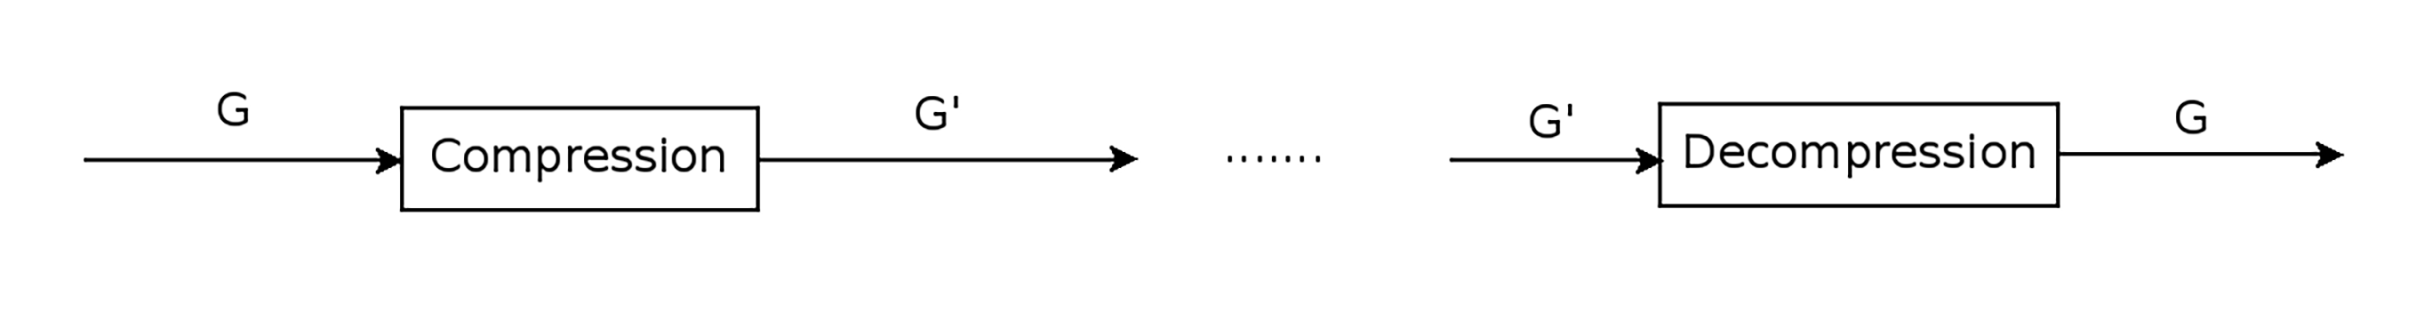
\includegraphics[scale=0.15,center]{./ressources/image/SansPerte.png}
			\caption[Compression sans perte.]{Compression sans perte.}
			\end{figure}
			
			%% citee qlq exemple de compression sans pertes
			
			\subsubsection{Compression Avec Perte:}
			Contrairement à la compression sans perte, la compression avec perte permet la suppression permanente de certaines informations jugées inutile (redondantes) pour améliorer la qualité de la compression.  En d'autres termes, le graphe G subi des transformations pour avoir une représentation compacte G' qui lors de la décompression donne un graphe G'' probablement différent de G mais l'approximant le plus possible. La figure ci-dessous illustre cette définition.   
			
			\begin{figure}[h]
			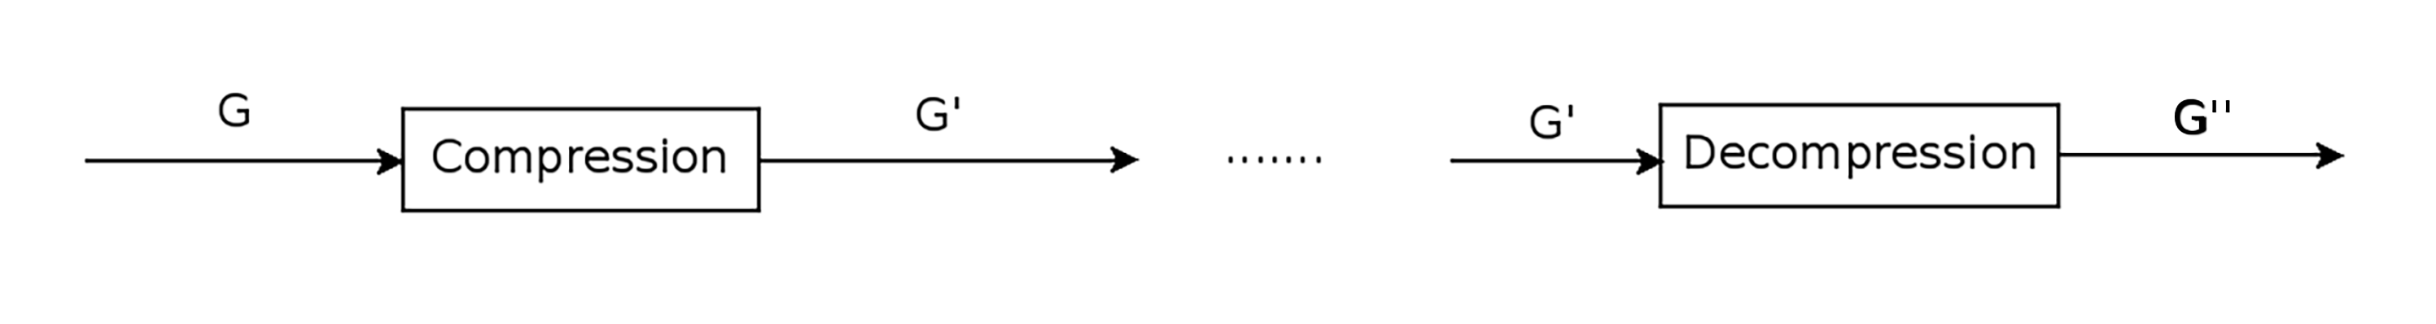
\includegraphics[scale=0.15,center]{./ressources/image/AvecPerte.png}
			\caption[Compression avec perte.]{Compression avec perte.}
			\end{figure}
			
			%%% citee qlq exemple de compression avec perte
			
	
			\subsection{Les métriques d'évaluation des algorithmes de compression:}
					
				Devant la panoplie d'algorithmes et de techniques de compression de graphe disponibles dans la littérature, des critères de comparaison  et d'évaluation entre ces méthodes doivent être bien définis. Dans cette partie nous présenterons les principaux mesures de performances.
				
				\subsubsection{Le temps de compression:}
				C'est une métrique qui donne le temps d'exécution de l'algorithme de compression. Elle est généralement mesurée en secondes (ou ms).
				\subsubsection{Le ratio de compression:}
				C'est la mesure la plus courante pour calculer l'efficacité d'un algorithme de compression. Il est défini comme le rapport entre le nombre total de bits requis pour stocker des données non compressées et le nombre total de bits nécessaires pour stocker des données compressées.
				%la formule
				\begin{center}
				$
				CR = \frac{No.\ de\ bits\ du\ graphe\ originale}{No.\ de\ bits\ du\ graphe\ finale }
				$
				\end{center}
				
				
				Le CR est parfois appelé bit par bit (bpb) et il est définit alors comme étant le nombre moyen de bits requis pour stocker les données compressées \citep{uthayakumar2018survey}. Dans le cas des algorithmes de compression de graphe on a:
				\begin{itemize}
					\item \textbf{Le nombre de bits par nœuds:}
					représente l'espace mémoire nécessaire pour stocker un nœud (bpn pour bits per node).
					%% la formule
					
					\item \textbf{Le nombre de bits par liens:}
					représente l'espace mémoire nécessaire pour stocker un liens (bpe pour bits per edge).
					%%la formule 
				\end{itemize}
				
				
				
				
				
				
				\subsubsection{Le taux de compression:}
				Exprimée en pourcentage, cette métrique permet de mesurer la performance de la méthode de compression. Elle peut être exprimer de deux manières différentes:
				
				\begin{itemize}
					\item \textbf{Le taux de compression:} Le rapport entre volume du graphe après compression et le volume initial du graphe.
					\begin{center}
				$
				t = \frac{La\ taille\ du\ graphe\ finale}{La\ taille\ du\ graphe\ originale }
				$
				\end{center}
					\item \textbf{Le gain d'espace: }Le gain d'espace représente la réduction de la taille du graphe compressé par rapport à la taille du graphe original.
					
					\begin{center}
				$
				G = 1 - \frac{La\ taille\ du\ graphe\ finale}{La\ taille\ du\ graphe\ originale }
				$
				\end{center}
					
					
				\end{itemize}
				
				
				%\subsubsection{L'erreur quadratique:}
			
			\subsection{Classification des méthodes de compression:}
			
		\section{Conclusion}
			
%--------->chapitre 03

\chapter{ Les méthodes de compression par extraction de motifs}
			
			La découverte de connaissances et l'exploration de données (KDD) ont pour objectif d'extraire des informations utiles à partir de sources de données, souvent sous la forme de modèles récurrents. Les motifs fréquents sont  des sous-graphes .
			
				
			\section{Compression par extraction de motifs}
			 Les motifs fréquents sont des connaissances extraites sur des données. Leur but est de fournir à l'utilisateur des informations non triviales, implicites, présumées non connues. Ils offrent ainsi à l'utilisateur une meilleure appréhension des données. L'extraction de motifs fréquents est ainsi devenue une tâche importante de la fouille de données et un thème très étudié par la communauté. Elle a aussi été vastement%%%% verifier ce mot
			 utilisée dans le domaine de compression des graphes vue qu'elle permet de ne garder que l'information utiles et d'éliminer les redondances de manière efficace. En effet, nous trouvons plusieurs méthodes basées sur ce principe dont nous proposons de les classifier en deux grandes classes: 
			 (i) les méthodes  de compression basées vocabulaire
			 (ii) les méthodes  de compression basées Agrégation.
			 
				Dans cette section, nous allons expliquer le principe de base de chaque classe où nous allons subdiviser chacune  en plusieurs sous-classe en se basant sur ce dernier. 
				%%% a revoir le dernier paragraphe
			 
				\subsection{Compression basée vocabulaire}
				Les méthodes de compression par extraction de motifs basées vocabulaire sont des méthodes qui ont attirées l'attention des chercheurs ces dernières années car elles permettent une meilleurs compréhension du graphe. Elles partent toujours d'un ensemble de structures prédéfinies qui ont été prouvées fréquent dans les graphes réels. Deux sous classes de cette dernières peuvent être d:
				 
					 \textbf{Basées sur des méthodes de clustering}
							
							Les méthodes de cette classe s'appuient sur le fait qu'on ne peut pas comprendre facilement les graphes denses, alors que quelques structures simples sont beaucoup plus faciles à comprendre et souvent très utiles pour analyser le graphe. Elles se basent sur des algorithmes de détection de communautés. 
							La question suivante peut alors se poser: pourquoi ne pas appliquer l'un des nombreux algorithmes de détection de communauté ou de partitionnement de graphe pour compresser le graphe en termes de communautés? La réponse est que ces algorithmes ne servent pas tout à fait le même objectif que la compression. Généralement, ils détectent de nombreuses communautés sans ordre explicite, de sorte qu'une procédure de sélection des sous-graphes les plus «importants» est toujours nécessaire. En plus de cela, ces méthodes renvoient simplement les communautés découvertes, sans les caractériser (par exemple, clique, étoile) et ne permettent donc pas à l'utilisateur de mieux comprendre les propriétés du graphe. 
							
							%Le partitionnement des graphes et la détection de communautés présentent un grand intérêt pour de nombreux domaines, notamment les sciences sociales, biologiques et Web. 
%			Ces dernières permettent d'obtenir des résumés de graphes diversifiés, chaque méthode étant orientée vers certains types de structures, telles que des cliques et des noyaux bipartites ou des étoiles. 
			Parmi les méthodes de détection les plus importantes dans la littérature nous trouvons :
			\begin{enumerate}
				\item \textbf{METIS\citep{karypis2000multilevel}}:est un schéma de partitionnement de graphe multiniveau basé sur la coupe basé sur la bissection récursive multiniveau (MLRB). Tant que la taille du graphe n'est pas sensiblement réduite, il grossit d'abord le graphe d'entrée en regroupant les nœuds dans des super-nœuds de manière itérative, de sorte que la coupe des bords soit préservée. Ensuite, le graphe grossi est partitionné à l'aide de MLRB et le partitionnement est projeté sur le graphe d'entrée G par le biais du retour en arrière. La méthode produit k partitions à peu près égales.
				\item \textbf{SPECTRAL\citep{hespanha2004efficient}}: partitionne un graphe en effectuant une classification en k-means sur les k premiers vecteurs propres du graphe d'entrée. L'idée derrière cette classification est que les nœuds avec une connectivité similaire ont des scores propres similaires dans les k premiers vecteurs.
				\item \textbf{LOUVAIN\citep{blondel2008fast}}:est une méthode de partitionnement basée sur la modularité pour détecter la structure de communauté hiérarchique. Comme SLASHBURN, LOUVAIN est itératif: (i) Chaque nœud est placé dans sa propre communauté. Ensuite, les voisins j de chaque nœud i sont pris en compte et i est déplacé vers la communauté j si le déplacement produit le gain de modularité maximum. Le processus est appliqué à plusieurs reprises jusqu'à ce qu'aucun gain supplémentaire ne soit possible. (ii) Un nouveau graphe est créé dont les super nœuds représentent les communautés et les super arêtes sont pondérés par la somme des poids des liens entre les deux communautés. L'algorithme converge généralement en quelques itérations.
				\item \textbf{SLASHBURN \citep{kang2011beyond}}:est un algorithme de ré-ordonnancement de nœud initialement développé pour la compression de graphes. Il effectue deux étapes de manière itérative: (i) il supprime les nœuds de haute centralité du graphe (ii) Il réorganise les nœuds de manière à ce que les identificateurs les plus petit soient attribués aux nœuds de degré élevé et les nœuds des composants déconnectés obtiennent les identificateurs les plus grands. Le processus est répété sur le composant connecté.
				\item \textbf{BIGCLAM\citep{yang2013overlapping}}:est une méthode de détection de communauté à chevauchement évolutive. Il est construit sur le constat que les chevauchements entre les communautés sont étroitement liés. En modélisant explicitement la force d’affiliation de chaque couple nœud-communauté, un facteur latent non négatif est attribué à cette dernière, qui représente le degré d'appartenance à la communauté. Ensuite, la probabilité d'un bord est modélisée en fonction des affiliations de communautés partagées. L’identification des communautés de réseau est réalisée en adaptant BIGCLAM à un réseau non dirigé donné G.
				\item \textbf{HYCOM\citep{araujo2014beyond}}:est un algorithme sans paramètre qui détecte les communautés à structure hyperbolique. Il se rapproche de la solution optimale en détectant de manière itérative les communautés importantes. L'idée clé est de trouver dans chaque étape une communauté unique qui minimise une fonction d'objectif basée sur la MDL en fonction des communautés précédemment détectées. La procédure itérative comprend trois étapes: les candidats à la communauté, la construction de la communauté et la déflation matricielle.
				
			\end{enumerate}
			
			%%%%%Un tableau Comparative
			 Nous présenterons dans ce qui suit une étude comparative entre ces méthodes dans le but de mieux comprendre leurs influence sur les méthode de compression.
			 \begin{table}[h]
							\footnotesize
							\begin{tabular}{|R{2cm}||C{1cm}|C{1.5cm}|C{1.5cm}|C{1.5cm}|C{1.5cm}|C{1.5cm}|C{2.5cm}|}
								\hline & Chevau-che-ment & Clique & Étoile & sous-graphe Bipartie & Chaîne & Structure Hyperbolique & Complexité \\
								\hline \textbf{Metis} & \textcolor{red}{\xmark} & \textcolor{PineGreen}{Beaucoup} & \textcolor{BurntOrange}{certaines} & \textcolor{BurntOrange}{certains} & \textcolor{red}{peu}  & \textcolor{red}{peu}  & O(m·k)\\
								\hline	\textbf{Spectral} & \textcolor{red}{\xmark} & \textcolor{PineGreen}{Beaucoup} & \textcolor{BurntOrange}{certaines} & \textcolor{PineGreen}{Beaucoup} & \textcolor{red}{peu}  & \textcolor{red}{peu}  & O($n^3$)\\
								\hline \textbf{Louvain} & \textcolor{red}{\xmark} & \textcolor{PineGreen}{Beaucoup} & \textcolor{BurntOrange}{certaines} & \textcolor{red}{peu}  & \textcolor{red}{peu}  & \textcolor{red}{peu} & O($n log n$)\\
								\hline \textbf{SlashBurn} & \textcolor{PineGreen}{\checkmark} & \textcolor{PineGreen}{Beaucoup} & \textcolor{PineGreen}{Beaucoup} & \textcolor{BurntOrange}{certains} & \textcolor{red}{peu} & \textcolor{red}{peu} & O(t($m+nlogn$)) \\
								\hline \textbf{Bigclam} & \textcolor{PineGreen}{\checkmark}  & \textcolor{PineGreen}{Beaucoup} & \textcolor{BurntOrange}{certaines} & \textcolor{red}{peu}  & \textcolor{red}{peu}  & \textcolor{red}{peu}  & O(d · n · t)\\					
								\hline \textbf{Hycom} & \textcolor{PineGreen}{\checkmark}  & \textcolor{BurntOrange}{certaines} & \textcolor{PineGreen}{Beaucoup} & \textcolor{BurntOrange}{certains} & \textcolor{red}{peu}  & \textcolor{PineGreen}{Beaucoup}  & O($k(m + h log h^2 +hm_{h} )$)\\
								
								
								
								\hline \textbf{KCBC} & \textcolor{PineGreen}{\checkmark} & \textcolor{PineGreen}{Beaucoup} & \textcolor{BurntOrange}{certaines} & \textcolor{red}{peu}  & \textcolor{red}{peu}  & \textcolor{red}{peu}  & O(t(m + n))\\
								
								\hline 
							\end{tabular} \\
								\caption{Tableau comparative entre les méthodes de clustering avec n = nombre de nœuds, m = nombre d'arêtes, k = nombre de clusters, t = nombre d'itérations, d = degré moyen de nœuds, h($m_{h}$) = nombre de nœuds (arêtes) dans la structure hyperbolique.}
    								\label{tab:clusteringMethode} 
							\end{table}
							\normalsize	
			 
							%%VOG*

Une première technique de compression usant de ces méthodes s'intitule VOG \citep{koutra2015summarizing}. C'est une méthode de base sur laquelle s'appuient toutes les autres méthodes de cette classe. Elle permet de compresser un graphe statique non orienté G à l'aide d'un vocabulaire de sous-structures qui apparaissent fréquemment dans les graphes réels et ayant  une signification sémantique, tout en minimisant le cout du codage en utilisant le principe de longueur de description minimale (MDL)\footnote{MDL est un concept de la théorie de l'information permettant de trouver le modèle ayant une longueur minimale: \textit{min}(\textit{D},\textit{M}) = L(\textit{M}) + L(\textit{D} | \textit{M}) où L(\textit{M}) est la longueur du modèle et L(\textit{D} | \textit{M}) est la longueur en bits de la description des donnés en utilisant le modèle \textit{M}.}. 
%Soit un graphe non orienté G(V,E), sans boucle avec n nœuds et m arêtes et soit A sa matrice d'adjacence. le résultat de VoG est une liste ordonnée de structures notés \textit{M}, on note par 
Le vocabulaire $\Omega$ utilisé est composé de six structures qui sont : clique (\textit{fc}) et quasi-clique (\textit{nc}), noyau bipartie (\textit{cb}) et quasi-noyau bipartie (\textit{nb}), étoile (\textit{st}) et chaine (\textit{ch}). On peut avoir un chevauchement au niveau des nœuds, les liens quand à eux sont pris selon un ordre FIFO et ne peuvent pas se chevauchés, i.e la première structure $ s \in \textit{M} $ qui décrit l'arête dans A détermine sa valeur.

On note par $\mathcal{C}_{x}$ l'ensemble de tous les sous-graphes possibles de type $x \in \Omega$, et $\mathcal{C}$ l'union de tous ces ensembles, $\mathcal{C}$ = ${\cup}_{x}\mathcal{C}_{x}$. La famille de modèles noté $\mathcal{M}$ représente tous les permutations possibles des éléments de $\mathcal{C}$. Par MDL, on cherche $\textit{M} \in \mathcal{M}$ qui minimise le mieux le cout de stockage du modèle et de la matrice d'adjacence.
En d'autre terme, VoG formule le problème de compression comme un problème d'optimisation dont la fonction objective est :
 \textit{min}(\textit{D},\textit{M}) = L(\textit{M}) + L(E) avec E= A $\bigoplus$ $\mathbf{M} $ représentant l'erreur. 

Pour l'encodage du modèle, on a pour chaque $\textit{M} \in  \mathcal{M}$ : 

\begin{center}
L(\textit{M}) = $L_{\mathbb{N}}$(|M|+1) + log $\left( \begin{array}{c}
|\textit{M}| + |\Omega\| -1 \\
|\Omega| -1 \\
\end{array} \right)$ + $\sum\limits_{s  \in \textit{M}} ( - log Pr(x(s)  |  \textit{M} ) + L(s) )$\\
\end{center}

Le premier terme représente le nombre de structures dans le modèle avec %$L_{\mathbb{N}}$
, le second terme encode le nombre de structures par type $x \in \Omega$ tant dis que le troisième terme permet  pour chaque structure $s \in \textit{M}$, d'encoder son type x(s) avec un code de préfixe optimale et d'encoder sa structure. Le codage des structures se fait selon leurs types :
%----------------------------------------------------------------
%----------------------------------------------------------------
%----------------------------------------------------------------

\textbf{Clique :} Pour l'encodage d'une clique, on calcule le nombre de nœuds de celle-ci, et on encode leurs ids :
L(\textit{fc}) = $L_{\mathbb{N}}$(|\textit{fc}|) + log ${n}\choose{|f_{c}|}$
%----------------------------------------------------------------
%----------------------------------------------------------------
%----------------------------------------------------------------

\textbf{Quasi-Clique :} Les quasi cliques sont encodées comme des cliques complètes, toute en identifiant les arêtes ajoutées dont le nombre est ||\textit{nc}|| et manquantes dont le nombre est noté ||\textit{nc}||' en utilisant des codes de préfixe optimaux : 
L(\textit{nc}) = $L_{\mathbb{N}}$(|\textit{nc}|) + log ${n}\choose{|n_{c}|}$ + log(|\textit{nc})|) + ||\textit{nc}||\textit{$l_{1}$} +  ||\textit{nc}||'\textit{$l_{0}$}
où \textit{$l_{1}$} = - log(||\textit{nc}||/(||\textit{nc}||+||\textit{nc}||')) et analogique à \textit{$l_{0}$} sont les longueurs des codes de préfixe optimaux des arêtes  ajoutées et manquantes.
%----------------------------------------------------------------
%----------------------------------------------------------------
%----------------------------------------------------------------

\textbf{Noyau bipartie :} notant par A et B les deux ensembles du noyau bipartie. On encode leurs tailles, ainsi que les identifiants de leurs sommets : 
L(\textit{fb}) = $L_{\mathbb{N}}$(|\textit{A}|) + $L_{\mathbb{N}}$(|\textit{B}|) + log ${n}\choose{|A|}$ + log ${n-|A|}\choose{|B|}$.
%----------------------------------------------------------------
%----------------------------------------------------------------
%----------------------------------------------------------------

\textbf{Quasi-Noyau bipartie :} Comme les quasi-cliques, les quasi-noyaux bipartie sont codés comme suit :
L(\textit{nb}) = $L_{\mathbb{N}}$(|\textit{A}|) + $L_{\mathbb{N}}$(|\textit{B}|) + log ${n}\choose{|A|}$  + log ${n-|A|}\choose{|B|}$+log(|area(\textit{nb})|) + ||\textit{nb}||\textit{$l_{1}$} + ||\textit{nb}||'\textit{$l_{0}$}.
%----------------------------------------------------------------
%----------------------------------------------------------------
%----------------------------------------------------------------

\textbf{Étoile :} L'étoile est un cas particulier d'un noyau bipartie. D'abord on calcule la nombre de spokes de l'étoile, ensuite on identifie le hub parmi les n sommets et les spokes parmi les n-1 restants.
L(\textit{st}) = $L_{\mathbb{N}}$(|\textit{st}|-1) +  log n + log ${n-1}\choose{|st|-1}$.
%----------------------------------------------------------------
%----------------------------------------------------------------
%----------------------------------------------------------------

\textbf{Chaine :} On calcule d'abord le nombre d'éléments de la chaine, ensuite on encode les identifiants des nœuds selon leurs ordre dans la chaine :
L(\textit{ch}) = $L_{\mathbb{N}}$(|\textit{ch}| - 1) + $\sum\limits_{i=0}^{|\textit{ch}|} ( n - i )$

%----------------------------------------------------------------
%---------------------La matrice de l'erreur----------------------
%----------------------------------------------------------------
\textbf{Matrice d'erreur :} la matrice d'erreur E est encodée sur deux parties $E^{+}$ et $E^{-}$. $E^{+}$  correspond à la partie de A que M modélise en rajoutant des liens non existants contrairement à $E^{-}$ qui représente les parties de A que M ne modélise pas. Notons que les quasi-cliques et les quasi-noyaux bipartie ne sont pas inclut dans la matrice d'erreur puisqu'ils sont encodés exactement donc on les ignorent. Le codage de $E^{+}$ et $E^{-}$ est similaire à celui des quasi-cliques, on a :
\begin{center}
L(${E}^{+}$) = log(|${E}^{+}$|) + ||${E}^{+}$||\textit{$l_{1}$} + ||${E}^{+}$||'\textit{$l_{0}$}\\
L(${E}^{-}$) = log(|${E}^{-}$|) + ||${E}^{-}$||\textit{$l_{1}$} + ||${E}^{-}$||'\textit{$l_{0}$}\\
\end{center} 
Pour la recherche du meilleur modèle $ \textit{M} \in \mathcal{M} $ , VoG procède sur trois étapes :
%---------------------------------------------------
%---------------------etape 01----------------------
%---------------------------------------------------
\begin{enumerate}
 \item \textbf{Génération des sous-structures }: Dans cette phase, Les méthodes de détection de communautés et de clustering sont utilisées pour décomposer le graphe en sous-graphes pas forcément disjoints. La méthode de décomposition utilisée dans VOG est SlashBurn.  
%---------------------------------------------------
%---------------------etape 02----------------------
%---------------------------------------------------
 \item \textbf{Étiquetage des sous-graphes }: L'algorithme cherche pour chaque sous-graphe généré dans l'étape précédente la structure $x \in \Omega$ qui le décrit le mieux, en tolérant un certain seuil d'erreur.
  \begin{enumerate}[label=\alph*]
     \item \textbf{Étiquetage des structures parfaites} : Tout d'abord, le sous-graphe est testé pour une similarité sans erreur par rapport aux structures complètes du vocabulaire :
		%----------------------------------------------------
		%---------------------etape 2.1----------------------
		%----------------------------------------------------
\begin{itemize}[label=$\circ$]
	\item si tous les sommets d'un sous graphe d'ordre n ont un degré égale à n-1, il s'agit alors d'une clique.
	\item si tous les sommets ont un degré de 2 sauf deux sommets ayant le degré 1, le  sous-graphe est une chaine.
	\item si les amplitudes de ses valeurs propres maximales et minimales sont égaux, le sous-graphe est un noyau bipartie où les sommet de chaque nœuds sont identifiés à travers un parcours BFS avec coloration des sommets.
	\item  Quant à l'étoile, elle est considérée comme un cas particulier d'un noyau bipartie, il suffit donc que l'un des ensembles soit composé d'un seule sommet.
\end{itemize}     
		%----------------------------------------------------
		%---------------------etape 2.2----------------------
		%----------------------------------------------------
     \item \textbf{Étiquetage des structures approximatives }: Si le sous graphe ne correspond pas à une structure complète, on cherche la structure qui l'approxime le mieux en terme du principe MDL.
     
  \end{enumerate} 
 % \textbf{Remarque} : Pour les structure parfaites, en plus du cout d'encodage de la structure, on rajoute le cout de l'erreur local c'est a dire, L($x^{*}$) + L($\textit{E}^{+}_{x^{*}}$) + L($\textit{E}^{-}_{x^{*}}$) où L($x^{*}$) est la description de la structure, L($\textit{E}^{+}_{x^{*}}$) et L($\textit{E}^{-}_{x^{*}}$) sont les arêtes incorrectement modélisés et les arêtes non  modélisés respectivement dans area($x^{*}$).
  
  
Après avoir représenter le sous graphe sous forme d'une structure, on l'ajoute à l'ensemble des structure candidates $\mathcal{C}$, en l'associant à son cout.

\item \textbf{Assemblage du modèle }: Dans cette dernière étape, une sélection d'un ensemble de structures parmi ceux de $\mathcal{C}$ est réalisée. Des heuristiques de sélections sont utilisées car le nombre de permutations est très grand ce qui implique des calcules exhaustifs. Les heuristiques permettent d'avoir des résultats approximatives et rapides, parmi les heuristiques utilisées dans VOG on trouve :
\begin{itemize}
\item PLAIN : Cette heuristique retourne toutes les structures candidates. e.i. \textit{M}= $\mathcal{C}$.
\item TOP-K :  Cette heuristique sélectionne les k meilleurs candidats en fonction de leurs gain en bits.
\item GREEDY'N FORGET(GNF) : Parcours structure par structure dans l'ensemble $\mathcal{C}$ ordonné selon la qualité (gain en bits), ajoute la structure au modèle tant qu'elle n'augmente pas le cout total de la représentation, sinon l'ignore.
%matnsaych kayn réf ta3had la méthode w matnsaych aussi réf ta3 mdl
\end{itemize}  
\end{enumerate}

%Ci-dessous le pseudo algorithme de VOG :

%\begin{algorithm}
%\caption{Pseudo Algorithme VOG}\label{euclid}
%\begin{algorithmic}[1]
%	\STATE \textbf{Entré :} Graphe G.
%	\STATE \textbf{Étape 1 :}  Génération des sous-graphe en utilisant une méthode de décomposition.  
%	\STATE \textbf{Étape 2 :} Étiquetage des sous graphe en choisissant la structure $x \in \Omega$ qui représente chaque sous- graphe avec le moindre coût.
%	\STATE \textbf{Étape 3 :} Assemblage des sous graphes en utilisant des heuristiques pour sélectionner un sous-ensemble non-redondant à partir des structure candidate de l'étape 2.
%	\STATE \textbf{Sortie :} Modèle \textit{M} et son cout d'encodage.
%\end{algorithmic}
%\end{algorithm}






							%%%VoG Overlapp
			Comme nous l'avons déjà précisé, VOG formule le problème de compression de graphe en tant que problème d'optimisation basé sur la théorie de l'information, l'objectif étant de rechercher les sous structures  qui minimisent la longueur de description globale du graphe. Un élément clé de VoG est la méthode de décomposition utilisée qui peut donner en sortie des sous-graphes ayant des nœuds et/ou des arêtes en commun et dont VoG\citep{koutra2015summarizing} ne suppose que le premiers cas. 
			En partant de ce constat, les auteurs de \citep{liu2015empirical} proposent VoG-overlapp, une extension de VoG prenant en compte les chevauchements des structures sous forme d'une étude expérimentale de l'effet de diverses méthodes de décomposition sur la qualité de la compression.
			%%%Algorithme 01
			
			L'idée de base de VoG-overlapp est d'inclure une pénalité pour les chevauchements importants dans la fonction objective ce qui oriente le processus de sélection des structures vers la sortie souhaitée. Elle devient alors:
			\begin{center}
				$min\ L(G,M) = min\ \big\{L(M) + L(E) +\textbf{L(O)}\big\}$
			\end{center}
			
			Le principe de calcul de $L(M)\ et\ L(E)$ demeure le même, avec O une matrice cumulant le nombre de fois que chacune des arêtes a été couverte par le modèle. Le cout du codage de la matrice des chevauchements est donné par la formule \eqref{eq:Lo}.
			\begin{equation} \label{eq:Lo}
				L(O) = log(|O|)\ +\ ||O||\ l_{1}\ +\ ||O||'\ l_{0}\ +\  \displaystyle{\sum_{o\in\varepsilon(O)}L_{N}(|o|)}
			\end{equation}
			Où :
			\begin{itemize}[label=$\circ$]
				\item $|O|$  est le nombre d'arêtes (distinctes) qui se répètent dans le modèles M. 
				\item $||O||$ et $||O||'$ représentent respectivement le nombre d'arêtes présentes et manquantes dans O.
				\item $l_{1} = -log (\frac{||O||}{||O||+||O||'})$, de manière analogique $l_{0}$, sont les longueurs des codes de préfixe optimaux pour les arêtes actuelles et manquantes, respectivement.
				\item $\varepsilon(O)$  est l'ensemble des entrées non nulles dans la matrice O.
			\end{itemize}
							Durant la même année, \citep{shah2015timecrunch} ont proposé une autre variation de VoG, TimeCrunch, pour le cas des graphes simples (sans boucles) non orientés dynamiques représentés par un ensemble de graphes associés chacun à timestamp. En d'autres termes, ils considèrent les graphes $\displaystyle{G=\bigcup_{t_{i}}G_{t_{i}}(V,E_{t_{i}})}\ \ 1 \preceq i \preceq t$ où $G_{t_{i}}$ = G a l'instant $t_{i}$.
			Un nouveau vocabulaire est proposé pour décrire proprement l'évolution des sous-structures dans le temps. En effet, ils partent du même vocabulaire de structures statiques 
			%citer les structures Ω = {st,fc,nc,bc,nb,ch}
			$\Omega =\{ st\ (etoile),\ fc (clique),\ nc (quasi-clique),\ bc (bipartie),\ nb (quasi-bipartie),\ ch (chaine)\}$ 
			dont ils affectent une signature temporelle $\delta \in \Delta$ où: $\Delta$ = \{o(oneshot), r(ranged), p(periodique), f(flickering), c(constante) \}. 
			
			 Comme les éléments du modèle sont modifiés, son cout est alors aussi modifié pour inclure pour chaque structure $s$ non seulement sa connectivité $c(s)$ correspondant aux arêtes des zones induites par $s$ mais aussi sa présence temporelle $u(s)$ correspondant aux timestamps dans lesquels $s$ apparait dans le graphe G. 
			 
			 $L(M) = L_{N}(|M|+1)\ +\ $log${|M|+|\Phi|-1}\choose{|\Phi|-1}$ $+\ \displaystyle{\sum_{s\in M}(logP(v(s)|M) + L(c(s)) + \textbf{L(u(s))})}$
			 
			 Le cout de l'encodage de la présence temporelle diffère selon ses caractéristiques. Nous présenterons dans ce qui suit la formule correspondant à chaque signature.
			 
			 \begin{itemize}[label=$\circ$]
			 \item \textbf{Oneshot}: cette signature décrit les sous-structure qui apparaissent dans un seul timestamp ,i.e $|u(s)|=1$. Donc le cout de l'encodage se réduit aux nombre de bits nécessaires pour sauvegarder le timestamp : $L(u(s)) = log(t)$.
			 \item \textbf{Ranged}: dans ce cas la sous-structure apparait dans tous les graphes se trouvant entre deux timestamps $t_{1}$ et $t_{2}$. Le cout englobe le nombre de timestamps dans lesquels elle apparait ainsi que les identifiants des deux timestamp $t_{debut}$ et $t_{fin}$ : $L(u(s)) = L_{N}(|u(s)|) +log$ ${t}\choose{2}$.
			 \item \textbf{Periodic}: cette catégorie est une extension   de la précédente avec les timestamps qui sont éloigné de plus d'un pas d'où: $L(p) = L(r)$.
			 
			 En effet, la périodicité peut être déduite des marqueurs début et de fin ainsi que du nombre de pas de temps $|u(s)|$, permettant ainsi de reconstruire $u(s)$
			 \item \textbf{Flickering}: ce type décrit les structures qui apparaissent dans $n$ timesteps de manière aléatoire. Le cout doit englober donc le nombre de timesteps ainsi que leurs identifiants d'où: 
			 $L(u(s)) = L_{N}(|u(s)|) +log$ ${t}\choose{|u(s)|}$.
			 \item \textbf{Constant}: dans ce cas la sous-structure apparait dans tout les timesteps et donc elle ne dépend pas du temps d'où L(c)=0.
			 \end{itemize}
			 
			 
			 Nous notons que décrire $u(s)$ est encore un autre problème de sélection de modèle pour lequel les auteurs tirent parti du principe MDL. En effet juste comme pour le codage de la connectivité, il peut ne pas être précis avec une signature temporelle donnée. Toutefois, toute approximation entraînera des coûts supplémentaires pour l'encodage de l'erreur qui englobent dans ce cas l'erreur de l'encodage de la connectivité ainsi que l'erreur de l'encodage de la signature temporelle.
			 
			 \begin{algorithm}
					\caption{TIMECRUNCH}
				\begin{algorithmic} [1]
					\STATE \textbf{Génération de sous-structure candidate: }Génération de sous-graphe pour chaque $G_{t_{i}}$ en utilisant un des algorithmes de décomposition de graphe statiques
					
					
					\STATE  \textbf{Étiquetage de sous-structure candidate: }Associer chaque sous-structure à une etiquette $x \in \Omega$ minimisant son MDL.
					
					\STATE  \textbf{Assemblage des sous-structures candidates temporelles :} Assembler les sous-structure des graphes $G_{t_{i}}$ pour former des structures temporelles avec un comportement de connectivité cohérente et étiquetez-les conformément en minimisant le coût de codage de la présence temporelle. Enregistrer le jeu de candidats $C_{x} \in C $.
					
					\STATE \textbf{Composition du graphe compressé: }Composition du modèle M d'importantes structures temporelles non redondantes qui résument G à l'aide des méthodes heuristiques VANILLA, TOP-10, TOP-100 et STEPWISE. Choisir M associé à l'heuristique qui génère le coût de codage total le plus faible.
				\end{algorithmic}
			\end{algorithm}
			 
			 
			 
			 
			 
			 
			 
			 
			 
			 
			 
			 
							Une dernière variante,
\newacronym{ConDenSe}{CONDENSE}{CONditional Diversified Network Summarization}
 s'intitulant \gls{ConDenSe}, a été présentée par Liu et al. \citep{liu2018reducing} où ils abordent efficacement trois contraintes principales des  méthodes précédentes: 
				(i) leurs dépendance à la méthode d'extraction de motifs 
				(ii) l'incapacité de certaines à gérer les motifs qui se chevauchent 
				(iii) leur dépendance vis-à-vis de l'ordre dans lequel les structures candidates sont considérées lors de la phase d'assemblage. En effet, pour résoudre le premier problème, ils combinent plusieurs méthodes d'extraction de motifs ce qui améliore la qualité des structures candidates en dépit  du temps d'exécution. Tant dis que pour répondre à la deuxième contrainte ils utilisent la fonction objective proposée dans \citep{liu2015empirical}. Arrivant à la dernière phase de l'algorithme, ils proposent quatre nouvelles heuristiques: 
				(1) STEP: choisie les K  meilleures structures, 
				(2) STEP-P: partitionne le graphe et affecte chaque motif  à la partition ayant un chevauchement maximal de nœuds avec lui. Ces partitions sont parcourues parallèlement pour ne prendre que la meilleure de toutes les structures dans chacune des partitions,
				(3) STEP-PA: amélioration de STEP-P en désignant chaque partition du graphe comme étant active, puis si une partition échoue x fois pour trouver une structure qui réduit le coût \gls{mdl} , cette partition est déclarée inactive et n'est pas visitée dans les prochaines itérations,
				 (4) K-STEP: combinaison des trois premières heuristiques. Il transforme par la suite chaque motif trouvé en un super-nœud.		
											\begin{landscape}
								\begin{table}
									\begin{tabular}{|c|c|c|c|c|c|c|c|c|c|c|c|c|}
										\hline
										& \multirow{2}{*}[-25pt]{Article}  & \multicolumn{4}{c|}{Graphe en entrée} & \multicolumn{2}{c|}{Compression} & \multicolumn{2}{c|}{Structure en sortie}  & \multirow{2}{*}[-25pt]{Graphe de test} & \multirow{2}{*}[-25pt]{Résultat}  \\ \cline{2-11}
				& \rotatebox[origin=c]{90}{ Orienté }  & \rotatebox[origin=c]{90}{ Non orienté } & \rotatebox[origin=c]{90}{ Statique } & \rotatebox[origin=c]{90}{ Dynamique } & \rotatebox[origin=c]{90}{ Avec perte } & \rotatebox[origin=c]{90}{ Sans perte } & \rotatebox[origin=c]{90}{ Succincte } & \rotatebox[origin=c]{90}{ Structurelle }  & & \\ \hline				%%%%%%Fin du header
										
										 \rotatebox[origin=c]{90} \multirow{4}{*}[-25pt]{Basé vocabulaire en utilisant les méthodes de clustering} & VoG \citep{koutra2015summarizing} & \xmark & \cmark & \cmark & \xmark & \xmark & \cmark & \cmark & \xmark  & 
	
	\begin{minipage}[t]{0.3\textwidth}
	ASOregon
    \begin{itemize}
    \item 13 milles nœuds
    \item 37 milles liens\\
    
    \end{itemize}
  \end{minipage}									 
			  & 71\%	\\

										 & VoG-Overlapp \citep{liu2015empirical}& \xmark & \cmark & \cmark & \xmark & \xmark &\cmark & \cmark & \xmark  &
										
	\begin{minipage}[t]{0.3\textwidth}
	ASOregon
    \begin{itemize}
    \item 13 milles nœuds
    \item 37 milles liens\\
    
    \end{itemize}
  \end{minipage}	
										 & 25\%	\\
										 & TimeCrunch \citep{shah2015timecrunch}& \xmark & \cmark & \cmark & \xmark & \xmark &\cmark & \cmark & \xmark & 

	\begin{minipage}[t]{0.3\textwidth}
	Enron
    \begin{itemize}
    \item 80 milles nœuds
    \item 288 milles liens\\
    
    \end{itemize}
  \end{minipage}											
										&74\%	\\
										 & CanDenSe \citep{liu2018reducing}&     \xmark & \cmark & \xmark & \cmark & \xmark  &\cmark & \cmark & \cmark &
\begin{minipage}[t]{0.3\textwidth}
	Enron
    \begin{itemize}
    \item 80 milles nœuds
    \item 288 milles liens\\
    
    \end{itemize}
  \end{minipage}											
										 &	 78\%\\
										\hline
									\end{tabular}
									\caption{Synthèse des méthode de compression par extraction de motifs basées sur des méthodes de clustering.}									
									
								\end{table}
								
							\end{landscape}
			
					 \textbf{Basée sur les propriétés de la matrice d'adjacence}
							
							Les graphes peuvent avoir différentes représentations. Chacune des structures de données présente des avantages et des inconvénients en ce qui concerne la quantité de mémoire nécessaire pour stocker les données et la facilité d'accès aux données. Selon les besoins, il est parfois utile de stocker les données dans des structures de données plus grandes, qui nécessitent plus d'espace mais offrent un accès efficace aux données. En se basant sur ce constat plusieurs méthodes ont été  proposée dans la littérature pour compresser la matrice d'adjacence en exploitant les propriété des graphes réels pour trouver les motifs les plus fréquent dans cette dernière.
							
							
	\citep{asano2008efficient} ont exploité les propriétés du graphe du web pour présenter une nouvelle méthode de compression (ECWG) sans perte permettant d'extraire les motifs à partir de la matrice d'adjacence. Il proposent un vocabulaire composée de six types de blocs (Motifs): un bloc horizontale de 1, un bloc verticale de 1, un bloc diagonale de 1, un rectangle de 1, un bloc de 1 sous forme de L et le singleton 1. Avant de procédé à l'extraction des motifs, la liste d'adjacence du graphe est partitionner selon les hôtes. Une nouvelle matrice d'adjacence est donc construite pour chaque hôte contenant les liens existants entre ses pages aux quel les liens inter-hote sont concaténés.
					Les blocs B sont détectés par la suite et chacun est représenté par un quadruplets (i, j, type(B), dim(B)) où i,j représentent les coordonnées du premier élément du blocs dans la matrice d'adjacence de l'hôte, type(B) représente le type du bloc et dim(B) représente les dimensions du bloc (omis dans le cas du singleton). 
					\begin{figure}[h]
					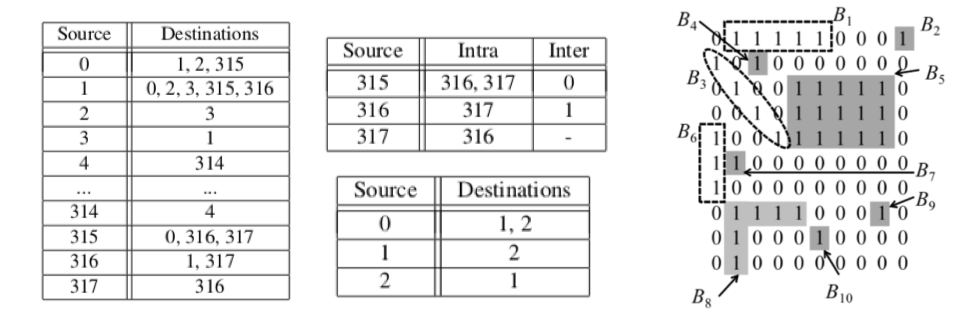
\includegraphics[scale=0.5]{ressources/image/inter_intra.png} 
					\caption{Exemple illustrant le principe de fonctionnement \citep{asano2008efficient}}
					\label{interIntra}
				\end{figure}
							
			Dans une méthode toute récente 
\newacronym{gcupmt}{GCUPMT}{Graph Compression Using Pattern Matching}			
			s'intitulant \gls{gcupmt}, Shah et Rushabh \citep{shah2018graph}  partitionnent les lignes de la matrice d'adjacence en plusieurs blocs ayant la même taille des motifs qui sont dans ce cas sous forme de vecteurs prédéfinies. Les blocs sont comparés avec l'ensemble des motifs ce qui entraîne , en cas de correspondance , le remplacement du bloc par un indicateur du motif précédé par un 1 indiquant que les bits suivants appartiennent à un indicateur de motif. Dans le cas contraire, les données brutes sont stockées directement précédées par un 0.
				
													\begin{landscape}
								\begin{table}
									\begin{tabular}{|c|c|c|c|c|c|c|c|c|c|c|c|c|}
										\hline
										\multirow{2}{*}[-25pt]{Article}  & \multicolumn{4}{c|}{Graphe en entrée} & \multicolumn{2}{c|}{Compression} & \multicolumn{2}{c|}{Structure en sortie}  & \multirow{2}{*}[-25pt]{Graphe de test} & \multirow{2}{*}[-25pt]{Résultat}  \\ \cline{2-11}
				& \rotatebox[origin=c]{90}{ Orienté }  & \rotatebox[origin=c]{90}{ Non orienté } & \rotatebox[origin=c]{90}{ Statique } & \rotatebox[origin=c]{90}{ Dynamique } & \rotatebox[origin=c]{90}{ Avec perte } & \rotatebox[origin=c]{90}{ Sans perte } & \rotatebox[origin=c]{90}{ Succincte } & \rotatebox[origin=c]{90}{ Structurelle }  & & \\ \hline				%%%%%%Fin du header
				
				\hline ECWG
 \citep{asano2008efficient}& \cmark & \cmark & \cmark & \xmark & \xmark &\cmark & \cmark & \xmark  &
										
	\begin{minipage}[t]{0.3\textwidth}
	uk-2002
    \begin{itemize}
    \item 18 millions de nœuds
    \item 298 millions liens\\
    
    \end{itemize}
  \end{minipage}	
										 & 76.1\%	\\
										
										\hline GCUPMT \citep{shah2018graph} & \cmark & \cmark & \cmark & \xmark & \xmark &\cmark & \cmark & \xmark & 
										
	\begin{minipage}[t]{0.3\textwidth}
	graphes avec :
    \begin{itemize}
    \item 8192 nœuds
    \\
    
    \end{itemize}
  \end{minipage}								 
			  & 70\%	\\

										\hline
									\end{tabular}
									\caption{Synthèse des méthode de compression par extraction de motifs basées vocabulaire exploitant les propriétés de la matrice d'adjacence.}									
									
								\end{table}
								
							\end{landscape}
					
				
				%%%%%%%%%%%%%%%%%%%%%%%%%%%%%%%%
				\subsection{Compression basée Agrégation des motifs}
				
					Les méthodes de compression par extraction de motifs basées sur l'agrégation sont des méthodes   qui agrègent plusieurs nœuds ou liens d'un motif en un seul nœud ou lien, appelés respectivement super-nœud et super-lien. Le graphe en sortie, dit super-graphe, devient dès lors plus simple et moins offrant ainsi une aisance et une facilité de traitement, d'exploration et de visualisation. 
					
					Nous présenterons dans ce qui suit les deux sous-classes de cette classe. 
					
					 
					\subsubsection{Compression basée Agrégation de nœuds}
					
					Les techniques de compression basées sur l'agrégation des nœuds des motifs sont des méthodes qui ont existé depuis plusieurs décennies offrant plusieurs avantages. 
					Elles visent à résumer le graphe initial en agrégeant les nœuds des motifs découvert dans le but de diminuer le nombre de nœuds existants  et d'offrir une meilleur visibilité et analyse du graphe. 
						
						Une première méthode de cette classe s'intitulent Subdue \citep{ketkar2005subdue}. Elle effectue une recherche \textit{Branch\&Bound} qui commence à partir de sous-structures composées de tous les sommets avec des étiquettes uniques. Les sous-structures sont prolongées de toutes les manières possibles par un sommet et une arête ou par une arête afin de générer des sous-structures candidates. Subdue conserve les instances de sous-structures et utilise l'isomorphisme de graphe pour déterminer les instances de la sous-structure candidate. Les sous-structures sont ensuite évaluées en fonction de leur compression de la longueur de description (DL) du jeu de données. Cette procédure se répète jusqu'à ce que toutes les sous-structures soient prises en compte ou que les contraintes imposées par l'utilisateur ne soient plus vérifiés. A la fin de la procédure, Subdue indique les meilleures sous-structures de compression.
				Le système Subdue fournit également la possibilité d'utiliser la meilleure sous-structure trouvée lors d'une étape de découverte pour compresser le graphe d'entrée en remplaçant ces instances de la sous-structure par un seul sommet et en effectuant le processus de découverte sur le  compressé. Cette fonctionnalité génère une description hiérarchique du jeu de données de graphe à différents niveaux d'abstraction en termes de sous-structures découvertes.
							
	\citep{rossi2018graphzip} partent de l'observation que les graphes réels sont formés souvent de nombreuses cliques de grande taille. En utilisant ceci comme base, GraphZip décompose le graphe en un ensemble de grandes cliques, qui est ensuite utilisé pour compresser et représenter le graphe de manière succincte. 
												\begin{landscape}
								\begin{table}
									\begin{tabular}{|c|c|c|c|c|c|c|c|c|c|c|c|c|}
										\hline
										\multirow{2}{*}[-25pt]{Article}  & \multicolumn{4}{c|}{Graphe en entrée} & \multicolumn{2}{c|}{Compression} & \multicolumn{2}{c|}{Structure en sortie} & \multicolumn{2}{c|}{Complexité} & \multirow{2}{*}[-25pt]{Graphe de test} & \multirow{2}{*}[-25pt]{Résultat}  \\ \cline{2-11}
				& \rotatebox[origin=c]{90}{ Orienté }  & \rotatebox[origin=c]{90}{ Non orienté } & \rotatebox[origin=c]{90}{ Statique } & \rotatebox[origin=c]{90}{ Dynamique } & \rotatebox[origin=c]{90}{ Avec perte } & \rotatebox[origin=c]{90}{ Sans perte } & \rotatebox[origin=c]{90}{ Succincte } & \rotatebox[origin=c]{90}{ Structurelle } & \rotatebox[origin=c]{90}{ Temporelle} & \rotatebox[origin=c]{90}{ Spaciale} & & \\ \hline				%%%%%%Fin du header
				
				\hline Subdue
 \citep{ketkar2005subdue}& \xmark & \cmark & \cmark & \xmark & \xmark & \cmark & \xmark & \cmark	 & & &		
	\begin{minipage}[t]{0.3\textwidth}
	Composante chimique :
    \begin{itemize}
    \item 21 étiquettes
    \item 422 transactions\\
    
    \end{itemize}
  \end{minipage}	
										 & 16\%	\\
										
										\hline GraphZip \citep{rossi2018graphzip} & \xmark & \cmark & \cmark & \xmark & \xmark & \cmark & \xmark & \cmark & & & 
				Web-Google						
								 
			  & 19\%	\\

										\hline
									\end{tabular}
									\caption{Synthèse des méthodes de compression par extraction de motifs basées agrégation de nœuds.}									
									
								\end{table}
								
							\end{landscape}
						
					\subsubsection{Compression basée agrégation de liens}
						Les méthodes de compression par extraction de motifs basées agrégation de liens sont parmi les méthode les plus populaires. Leur objectif est de produire un graphe compressé à partir du graphe initial en remplaçant les liens denses du graphe par un nouveau super-nœud ou une nouvelle super-arêtes. Elle se divise selon le principe en deux grandes classes: celles utilisant les règles de grammaire et celles utilisant des méthode de clustering. Nous détaillerons dans ce qui suit ces deux classes et nous conclurons par une synthèse sur les méthodes de chaque classe.
						
						 \textbf{Basées sur les règles de grammaire} 
								
								La classe des méthodes de compression basées sur les règles de grammaire est une généralisation d'une méthode de compression des dictionnaire s'intitulant Re-pair. Son principe de base consiste en la  recherche, à chaque itération, de la paire de symboles la plus fréquente dans une séquence de caractères et à la remplacer par un nouveau symbole, jusqu'à ce qu'il ne soit plus commode de les remplacer. Nous notons que dans ce cas le motif est sous forme de deux arêtes ayant un sommet en commun, nommé \textit{digraph}.
								
										Une première méthode de suivant ce principe a été proposée dans \citep{claude2010fast} baptisé \textit{Approximate Re-pair}. Dans cette méthode un graphe G=(V,E) est représenté sous forme d'une sequence de caractères T: \begin{center}
		T=T(G)= $\overline{v_{1}}\ v_{1,1}\ ...\ v_{1,a}\ \overline{v_{2}}\ v_{2,1}\ ...\ v_{2,a_{2}} ... \overline{v_{n}}\ v_{n,1}\ ...\ v_{n,a_{n}}\ $						
\end{center}	
où $\overline{v_{i}}$ représente un indicateur du sommet $v_{i}$. Elle procède en trois étapes essentielles expliquer dans l'algorithme \textbf{\ref{alg:re_pair}} .
	\begin{algorithm}
		\caption{Approximate Re-pair}
		\label{alg:re_pair}
		\begin{algorithmic}[1]
			\STATE \textbf{Calcule des fréquences:} T est parcourue séquentiellement et chaque pair $t_{i}t_{i+1}$ est ajouté à un tableau de hachage H avec leurs nombre d'occurence. 
			\STATE \textbf{Recherche des k meilleurs paires:}  H est parcourue et  les k paires les plus fréquentes sont retenues, en utilisant k pointeurs vers les cellules de H.
			\STATE \textbf{Le remplacement simultané:} les k paires identifiés dans l'étape précédente sont simultanément remplacées par un nouveau identifiant et une règle de production est ajoutée.
		\end{algorithmic}
	\end{algorithm}
	Lorsqu'il n'y a plus de paires à remplacer, Approximate Re-pair s'arrête donnant comme résultat un compressé compacte C de la chaine T. Pour finaliser le processus, tous les indicateurs de nœuds $\overline{v_{i}}$ seront supprimés de C. De plus, l'algorithme crée une table qui contiendra des pointeurs vers le début de la liste d'adjacence de chaque nœud dans C. Grâce à cette table l'algorithme pourra répondre aux requêtes de recherche de successeurs en un temps optimal.
								 %%%%exemple ???
								
	Dans un travail ultérieure \citep{claude2010extended} , les même auteurs s'intéressent aux requêtes de recherche des nœuds prédécesseurs et successeurs à partir du graphe compressé de \textit{Approximate Re-pair} directement. Il proposent alors de combiner leurs méthode avec une représentation basé sur les relations binaires de \citep{barbay2006adaptive}. En effet, ce dernier consiste à représenter les listes d'adjacence à l'aide d'une représentation séquentielle permettant de rechercher les occurrences d'un symbole puis de rechercher les voisins inverses à l'aide de cette primitive. 
								
Claude et Ladra \citep{claude2011practical} partagaient les mêmes préoccupations des auteurs de la méthode précédente et ont proposé comme solution de combiner la méthode Re-pair avec la représentation k2-tree. Ils obtiennent alors une compression de 2,27 (pbe) sur le graphe UK2002, tout en conservant la possibilité d'interroger les voisins entrants et sortants \citep{maneth2015survey}.
							
								
	Une dernière méthode de cette classe s'instituant gRepair a été proposé dans \citep{maneth2018grammar}. Ce nouveau algorithme de compression détecte de manière récursive des sous-structures répétées et les représente via des règles de grammaire.  Des requêtes spécifiques telles que l'accessibilité entre deux nœuds ou des requêtes de chemin normal peuvent ainsi être évaluées en temps linéaire (ou en temps quadratiques, respectivement), sur la grammaire, permettant ainsi des accélérations proportionnelles au taux de compression. la figure xxx presentent le resultat de cette methode sur un exemple. 
								%%%%exemple ???
																						\begin{landscape}
								\begin{table}
									\begin{tabular}{|C{3cm}|c|c|c|c|c|c|c|c|c|c|c|c|}
										\hline
										\multirow{2}{*}[-25pt]{Article}  & \multicolumn{4}{c|}{Graphe en entrée} & \multicolumn{2}{c|}{Compression} & \multicolumn{2}{c|}{Structure en sortie} & \multicolumn{2}{c|}{Complexité} & \multirow{2}{*}[-25pt]{Graphe de test} & \multirow{2}{*}[-25pt]{Résultat (bits/lien)}  \\ \cline{2-11}
				& \rotatebox[origin=c]{90}{ Orienté }  & \rotatebox[origin=c]{90}{ Non orienté } & \rotatebox[origin=c]{90}{ Statique } & \rotatebox[origin=c]{90}{ Dynamique } & \rotatebox[origin=c]{90}{ Avec perte } & \rotatebox[origin=c]{90}{ Sans perte } & \rotatebox[origin=c]{90}{ Succincte } & \rotatebox[origin=c]{90}{ Structurelle } & \rotatebox[origin=c]{90}{ Temporelle} & \rotatebox[origin=c]{90}{ Spaciale} & & \\ \hline				%%%%%%Fin du header
				
				\hline Approximate Re-pair
   \citep{claude2010fast}& \cmark & \xmark & \cmark & \xmark & \xmark &  \cmark & \cmark & \xmark	 & & &		
	\begin{minipage}[t]{0.3\textwidth}
	uk-2002 :
    \begin{itemize}
    \item 18 millions de nœuds
    \item 298 millions de liens\\
    
    \end{itemize}
  \end{minipage}	
										 & 4.23	\\

										\hline Approximate Re-pair \citep{claude2010extended} & \cmark & \xmark & \cmark & \xmark & \xmark & \cmark & \cmark & \xmark  & & & 
										\begin{minipage}[t]{0.3\textwidth}
	uk-2002 :
    \begin{itemize}
    \item 18 millions de nœuds
    \item 298 millions de liens\\
    
    \end{itemize}
  \end{minipage}	 & 3.98 \\ 
  			\hline gRe-pair \citep{maneth2018grammar} & \cmark & \cmark & \cmark & \xmark & \xmark & \cmark & \cmark & \xmark & & &
  				\begin{minipage}[t]{0.3\textwidth}
  			NotreDame :
    \begin{itemize}
    \item 325 milles de nœuds
    \item 1M de liens\\
  		\end{itemize}
  \end{minipage}		
  			& 4.84 \\\hline
									\end{tabular}
									\caption{Synthèse des méthodes de compression par extraction de motifs basées agrégation de liens en utilisant les règles de grammaire.}									
									
								\end{table}
								
							\end{landscape}
								

								
%%% Ajouter son algorithme
%%%% Ajouter un exmple illustant cette methode
								
						 \textbf{Basées sur des méthodes de clustering}
						 
						 		Les méthodes de compression appartenant à la classe courante sont des méthodes basées sur la recherche des sous-graphes denses (ayant des nœuds fortement connectés). Ils sont destinées principalement aux graphes du Web et les graphes des réseaux sociaux dans but de faciliter leurs exploration et analyse.
								
									%-----------------Aggregation des liens ----------%
				\citep{buehrer2008scalable} ont exploité l'existence de plusieurs ensembles de pages web qui ont les même liens sortants. S'intitulant  VNM pour Virtual Node Miner, leurs approche est basée sur la réduction du nombre de liens en créant des nouveaux sommets virtuels qui sont ajoutés au graphe. Soit G = (V,E) un graphe orienté, l'algorithme proposé se compose de deux phases essentielles :
				\begin{enumerate}
				
				
					\item \textbf{Phase de Clustering :}
					
					Le but de cette première étape est de contourner la tâche presque impossible d'extraction simultanée de centaines de millions de points de données en groupant d'abord les sommets similaires dans le graphes dans des clusters. 
				Pour cela k fonctions de hachage indépendantes sont utilisées pour obtenir une matrice de taille V * k. Par la suite, les lignes de la matrice  sont triées lexicographiquement
				%Ce tri est assez rapide car il ne nécessite que O (2V log V) en mémoire à la fois, ce qui tient dans la RAM (ou nous le faisons en minant le graphique en morceaux). 
				et elle est parcourue colonne par colonne en regroupant les lignes ayant la même valeur. Lorsque le nombre total de lignes chute au-dessous d'un seuil ou que le bord de la matrice de hachage est atteint, les identifiants des sommets associés aux lignes sont renvoyé au processus d'extraction (Phase 02). 
					
					\item \textbf{Phase d'Extraction de Motifs :}				Le but de cette étape est de localiser des sous-ensembles communs de liens sortants dans les sommets donnés. 
				Ainsi les ensembles plus grands et fréquents présentent un intérêt, car ils peuvent représenter des motifs plus pertinents et une meilleure compression. En effet, les performances de compression d'un motif  sont calculés en fonction de sa fréquence dans la liste d'adjacence, et de sa taille qui est le nombre de liens qu'il contient \eqref{eqcompperf}.
				%%% Formule
				\begin{equation}
				Compression(P)=(P.fréquence-1)(P.taille-1)-1
				\label{eqcompperf}
				\end{equation}
				Afin d'extraire ces motifs, VNM utilise une heuristique gloutonne. Cette heuristique procède comme suit :
				\begin{enumerate}
				\item Extraire un histogramme des identifiants de liaison sortante à partir de la liste d'adjacence des sommets données.
				\item Les listes sont réorganisées dans l'ordre décroissant des fréquences des liens sortants en éliminant ceux qui apparaissent une seul fois uniquement.
				\item Chaque lien sortant est ajouté à un arbre de préfixes avec l'ensemble trié de ces extrémités initiales selon leurs identifiants. 
				\item L'arbre est par la suite parcouru afin d'identifier les motifs qui maximisent la formule de performance de la compression \ref{eqcompperf}. Ces motifs sont ensuite convertis en nœuds virtuels et les identificateurs de sommet de leurs listes sont supprimés.
				\end{enumerate}
				 
				\end{enumerate}
				
				L'algorithme est appliqué jusqu'à ce que la réduction n'apporte pas un gain significative. La figure \ref{tab:VNM_exm} illustre le principe de fonctionnement de cette méthode sur un exemple.
				
				
			%%%%		Inclure un exemple 
			
		\begin{table}[h!]
			
		 \begin{flushleft}
			\begin{tabular}{C{4cm}||C{9cm} }
				 Phase 01 &  Phase 02 \\
				 {\renewcommand{\arraystretch}{0.6}
					\begin{tabular}[b]{R{0.4cm}|L{0.3cm} L{0.3cm} L{0.3cm}}
				 			id & \(\displaystyle h_{1}\)  & \(\displaystyle h_{2}\) &  \(\displaystyle h_{3}\) \\
							\hline  13 &\cellcolor{blue!25}10&\cellcolor{blue!25}11&\cellcolor{blue!25}12\\
							    	    23 &\cellcolor{blue!25}10&\cellcolor{blue!25}11&\cellcolor{blue!25}12\\
								   	43 &\cellcolor{blue!25}10&\cellcolor{blue!25}11&\cellcolor{blue!25}12\\
				  					55 &\cellcolor{blue!25}10&\cellcolor{blue!25}11&\cellcolor{blue!25}12\\
				  					64 & \cellcolor{blue!25}10&\cellcolor{blue!25}11&\cellcolor{blue!25}12\\
				  					102 &\cellcolor{blue!25}10&\cellcolor{blue!25}11&\cellcolor{blue!25}12\\
				  					204 &\cellcolor{blue!25}10&\cellcolor{blue!25}11&\cellcolor{blue!25}12\\
				  					431 &\cellcolor{blue!25}10&\cellcolor{blue!25}11&\cellcolor{blue!25}12\\
				  					480 &\cellcolor{blue!25}10&\cellcolor{blue!25}11&2\\
				  					501 &\cellcolor{blue!25}10&4&1\\
			\end{tabular}
				
				
				
				1. Calcul des fonctions de hachage et groupement des sommets			
			} &
			{
				 \begin{multicols}{2}
					\renewcommand{\arraystretch}{0.6}
 						 \begin{tabular}{R{0.4cm}|L{3.2cm} }
				 id &  liens sortants \\\hline
				  13 & 1 2 3 8\\
				  23 & 1 2 3 5 6 10 12 15 \\
				  43 & 1 2 3 5 6 10 22 31\\
				  55 & 1 2 3 5 \\
				  64 & 1 2 3 5 6 10 12 15 \\
				  102 & 1 2 3 20\\
				  204 & 1 7 8 9\\
				  431 & 1 2 3 4 5 6 10 22 31\\
			\end{tabular}
			
			
			2.1 la Liste d'adjacence.
			\columnbreak
 				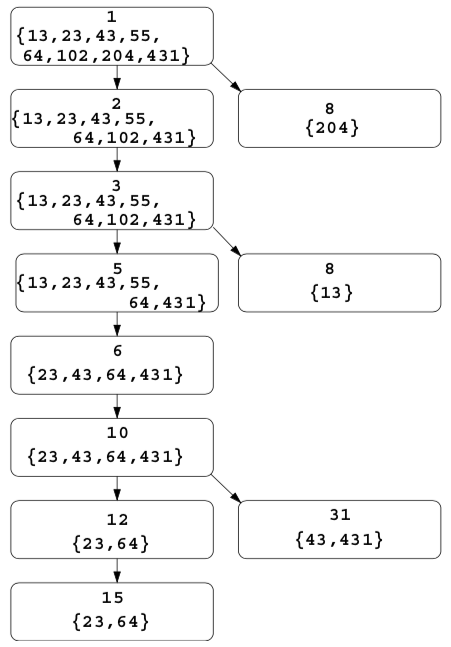
\includegraphics[scale=0.3]{ressources/image/VNM_exemple.png} 
 			%	2.2 Construction de l'arbre
 			
			\end{multicols}
			\begin{center}
		\renewcommand{\arraystretch}{0.6}
		\begin{tabular}{C{1cm} | C{1cm} L{4cm} C{1cm}}
			taille & freq & Liste des noeuds & Savings\\\hline
			6&4&43 431 23 64&14\\
			3&7&23 55 102 64 43 431&11\\
			8&2&23 64&6\\
			7&2&43 431&5\\
		
				\end{tabular}
				2.3 Extraction des Motifs
		\end{center}
			}
			
			\end{tabular}
		\end{flushleft}
		\caption{Exemple d'exécution de VNM}
   			 \label{tab:VNM_exm}
		\end{table}
		
		%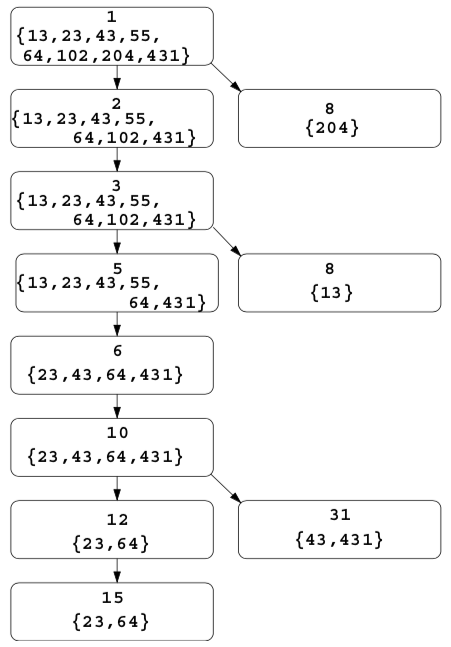
\includegraphics[scale=0.5]{ressources/image/VNM_exemple.png}
									Une variante de VNM a été proposée par Hernandez et Navarro \citep{hernandez2014compressed}. Comme première contribution, ils augmentent les types de structures découvertes dans la phase de clustering pour englober aussi: les cliques, les bi-cliques. L'extraction de motifs cette fois-ci n'est basée sur un parcours des feuilles vers la racine mais l'inverse où  l'ensemble des sommets finales des liens du motifs est constitués des étiquettes des nœuds de l'arbre inclus dans le chemin de la racine vers la feuille et  les sommets initiales sont la liste des sommets inclus dans le nœud feuille. 
				%%Noublie pas revient vers la source 
				Leurs deuxième contribution consiste en une hybridation dans le but de représenter le graphe en sortie à l'aide de structures compactes. Une première approche proposée est d'utiliser les  k2-trees \citep{brisaboa2009k} et qui donnent la représentation la plus compacte.  
				La deuxième hybridation consiste en une nouvelle structure proposée par les auteur.\\
				%revoire cela avec SAnna
				\begin{figure}[h]
					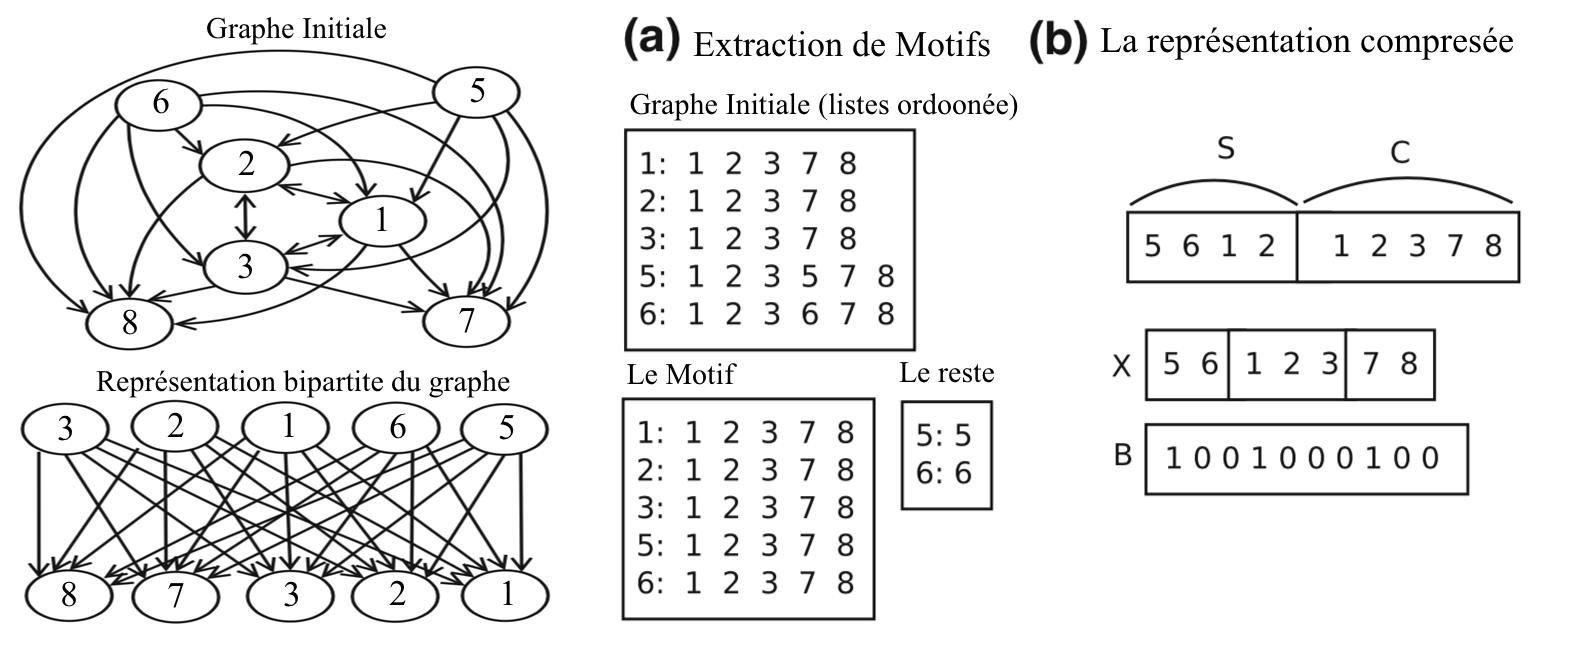
\includegraphics[scale=0.25]{ressources/image/VNM2_exemple.png} 
					\caption{Exemple d'exécution de SDM}
					\label{SDM}
				\end{figure}
										\begin{landscape}
								\begin{table}
									\begin{tabular}{|C{4cm}|c|c|c|c|c|c|c|c|c|c|c|c|}
										\hline
										\multirow{2}{*}[-25pt]{Article}  & \multicolumn{4}{c|}{Graphe en entrée} & \multicolumn{2}{c|}{Compression} & \multicolumn{2}{c|}{Structure en sortie}  & \multirow{2}{*}[-25pt]{Graphe de test} & \multirow{2}{*}[-25pt]{Résultat (bits/lien)}  \\ \cline{2-11}
				& \rotatebox[origin=c]{90}{ Orienté }  & \rotatebox[origin=c]{90}{ Non orienté } & \rotatebox[origin=c]{90}{ Statique } & \rotatebox[origin=c]{90}{ Dynamique } & \rotatebox[origin=c]{90}{ Avec perte } & \rotatebox[origin=c]{90}{ Sans perte } & \rotatebox[origin=c]{90}{ Succincte } & \rotatebox[origin=c]{90}{ Structurelle } & & \\ \hline				%%%%%%Fin du header
				
				\hline VNM
 \citep{buehrer2008scalable}& \cmark & \xmark & \cmark & \xmark & \xmark & \cmark & \xmark & \cmark &		
	\begin{minipage}[t]{0.3\textwidth}
	uk-2002 :
    \begin{itemize}
    \item 18 millions de noeuds
    \item 298 millions de liens \\
    
    \end{itemize}
  \end{minipage}	
										 & 1.95\	\\
										
										\hline DSM \citep{hernandez2014compressed} & \cmark & \xmark & \cmark & \xmark &  \xmark & \cmark & \cmark & \cmark  & 
				\begin{minipage}[t]{0.3\textwidth}
	uk-2002 :
    \begin{itemize}
    \item 18 millions de noeuds
    \item 298 millions de liens \\
    
    \end{itemize}
  \end{minipage}						
								 
			  & 1.53	\\

										\hline
									\end{tabular}
									\caption{Synthèse des méthodes de compression par extraction de motifs basées agrégation de liens en utilisant des heuristiques de clustering.}									
									
								\end{table}
								
							\end{landscape}
						
												
								
		\section{Conclusion}


%---->chapitre 03 :« Etude empirique »
	\chapter{Les méthodes de compression k2-Trees}
	
	
	
	
	
	%\begin{defn}
	%		Here is a new definition
	%\end{defn}
	

%Conclusion Générale									Obligatoire
\chapter{Conclusion} 

%Références Bibliographiques (fin de la pagination)		Obligatoire

%Annexes													Selon besoin


\newpage
\bibliography{Bibliographie}
\bibliographystyle{apalike}

\end{document}

%\renewcommand{\thefigure}{\arabic{figure}}
%\setcounter{figure}{0}
%\begin{figure}[H]
%	\centering
%	\includegraphics[scale=1]{ressources/image/LAAS-2016.jpg}
%	\label{fig:figure1}
%	\caption{This is a teste of figure}
	
%\end{figure}








